\begin{figure}[H]
\centering
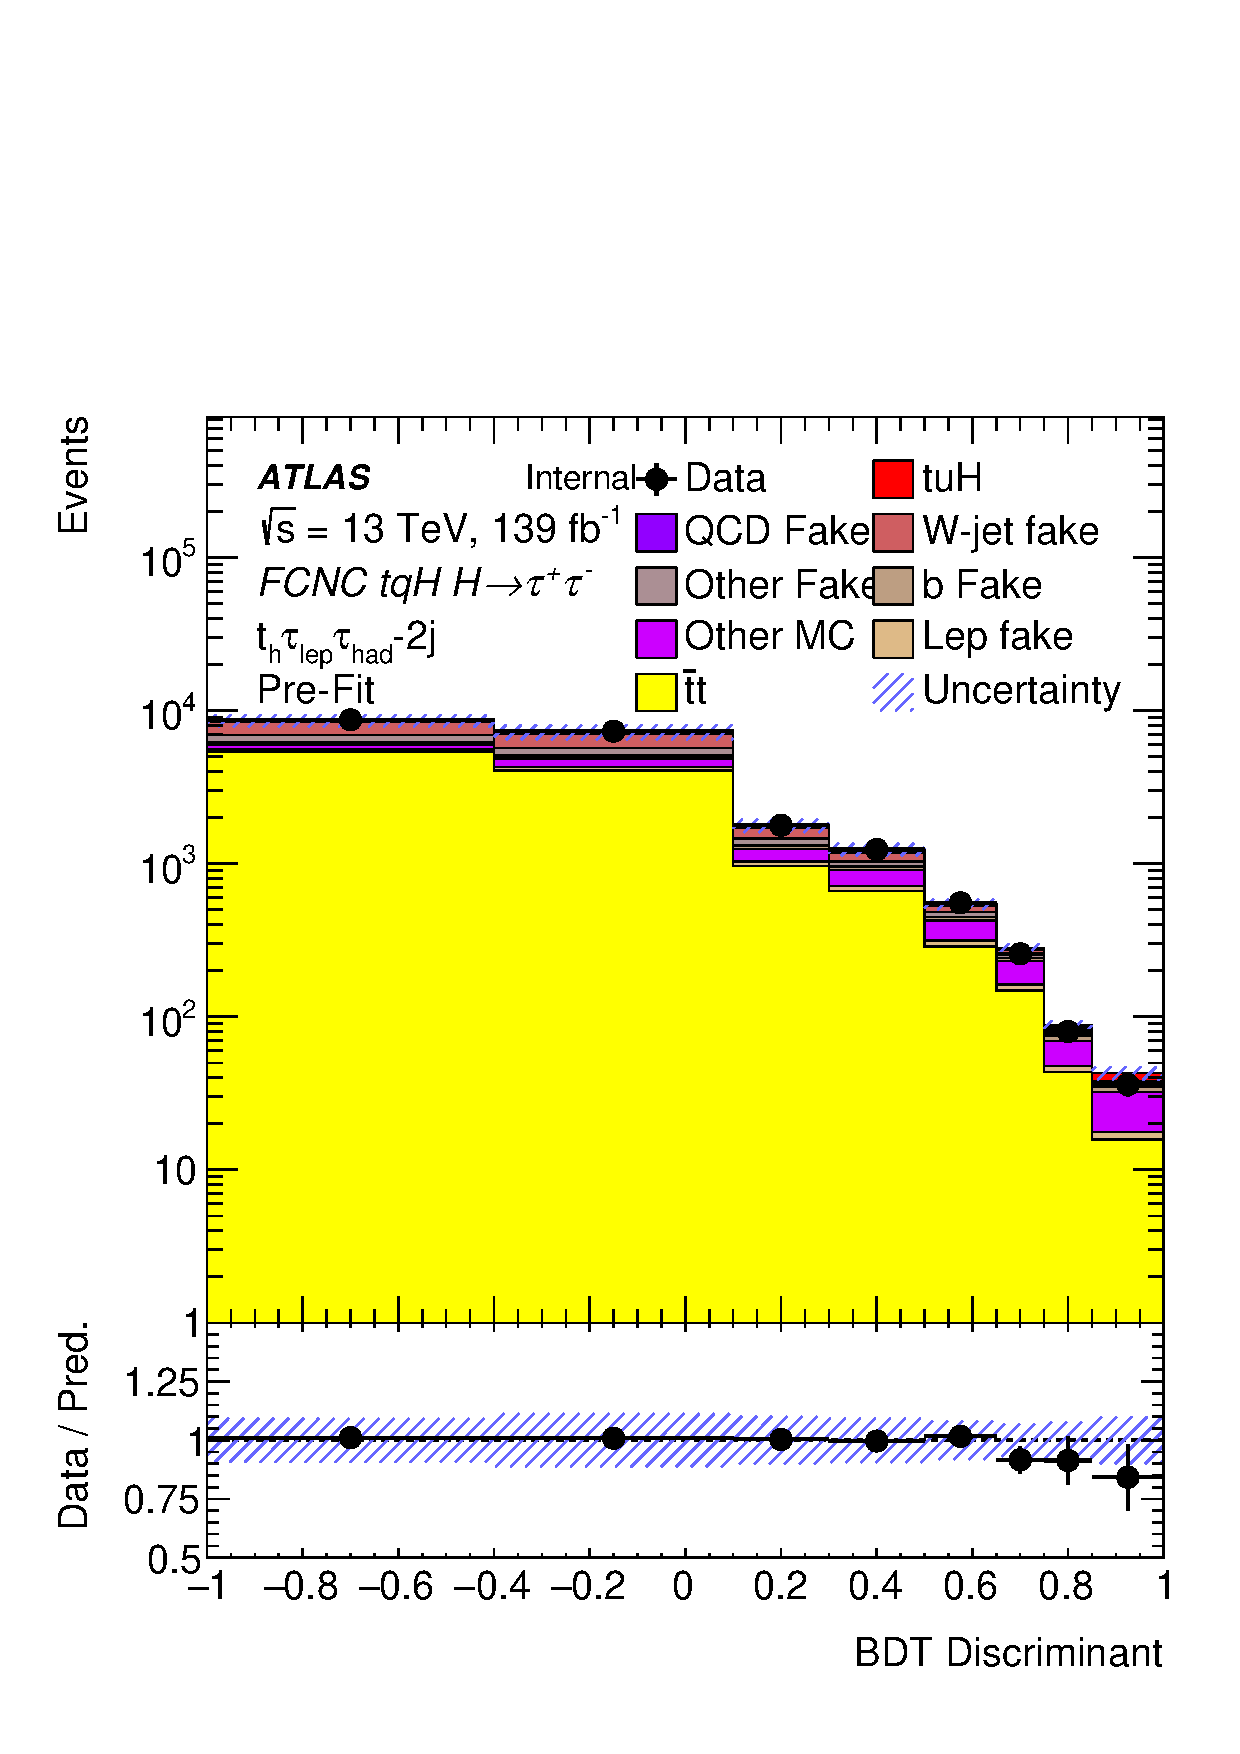
\includegraphics[width=0.30\textwidth]{\FCNCFigures/tthML/Limit/tuH_reg1l1tau1b2j_os.pdf}
\put(-100, 55){\textbf{(a1)}}
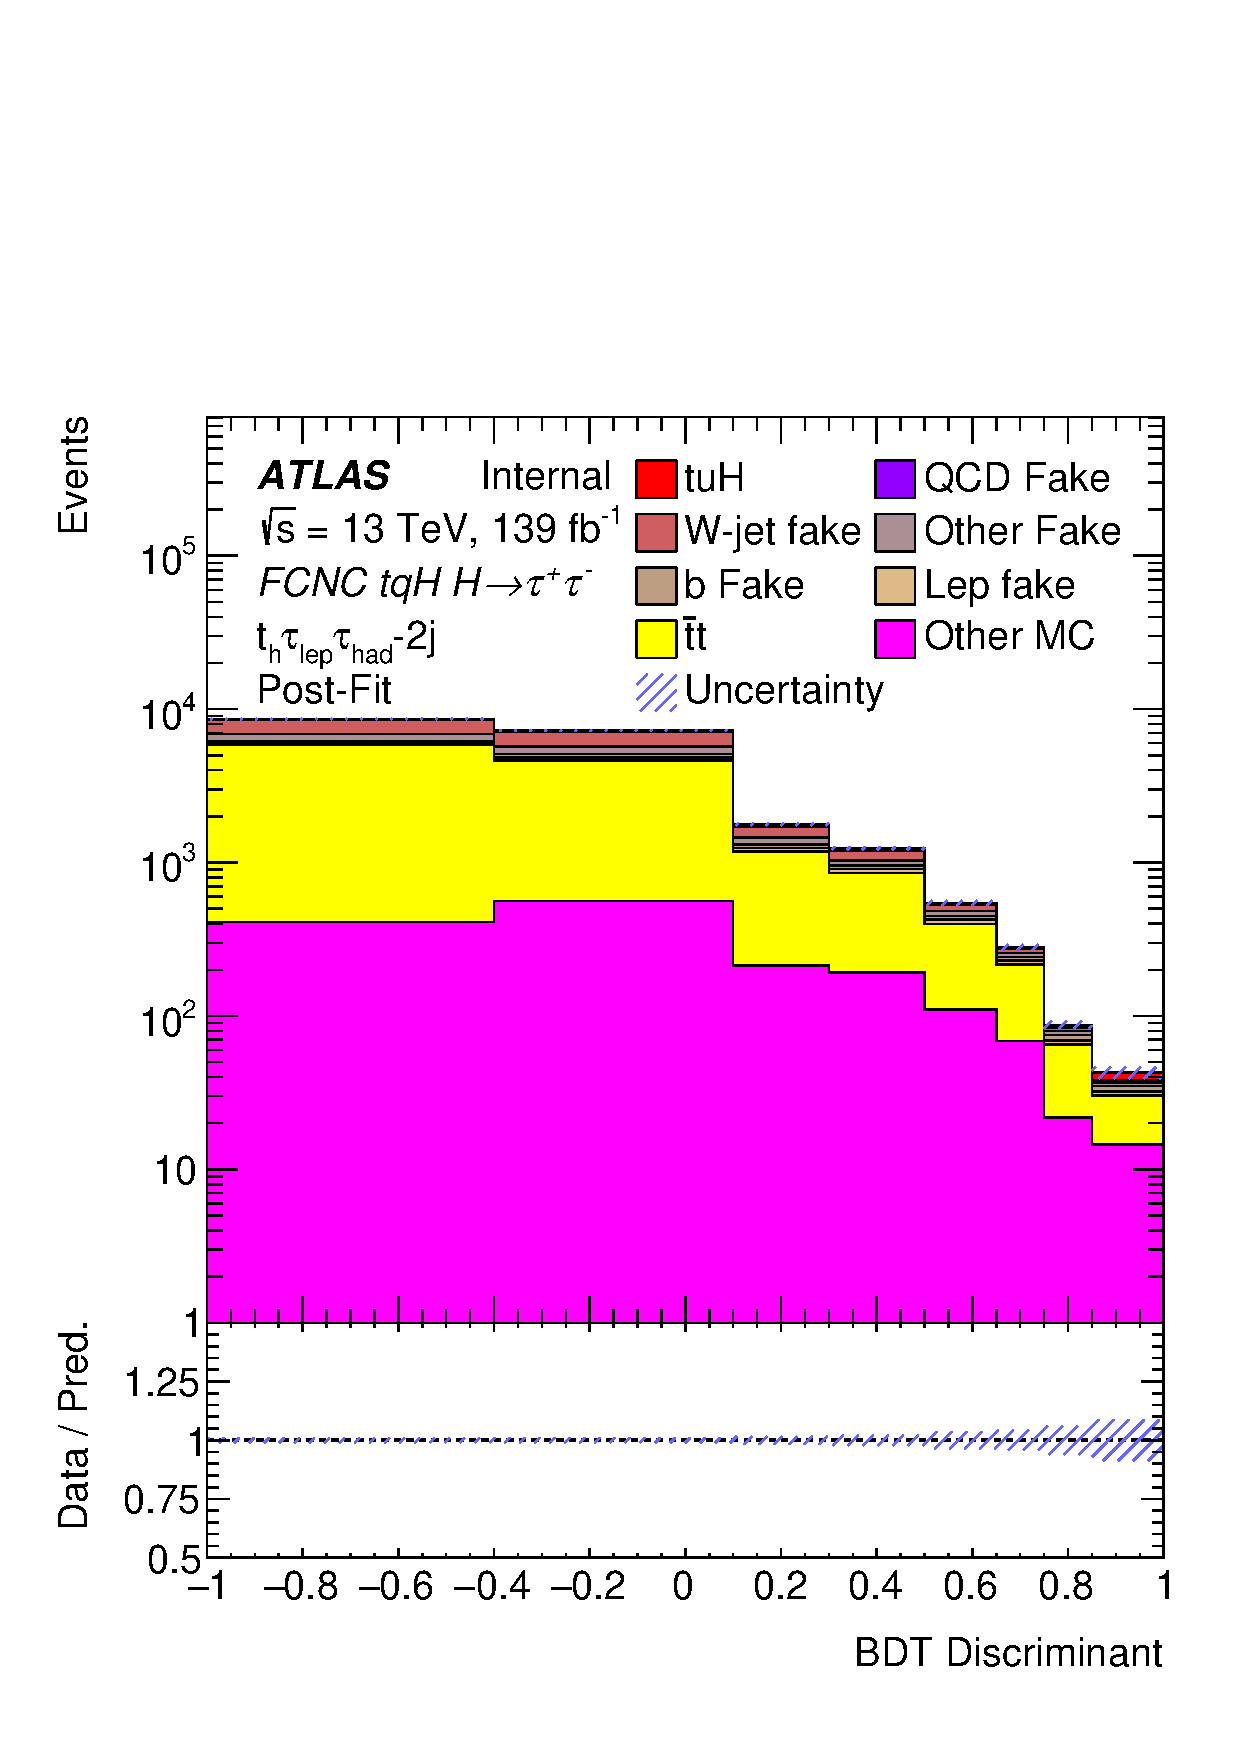
\includegraphics[width=0.30\textwidth]{\FCNCFigures/tthML/Limit/tuH_reg1l1tau1b2j_os_postFit.pdf}
\put(-100, 55){\textbf{(a2)}}
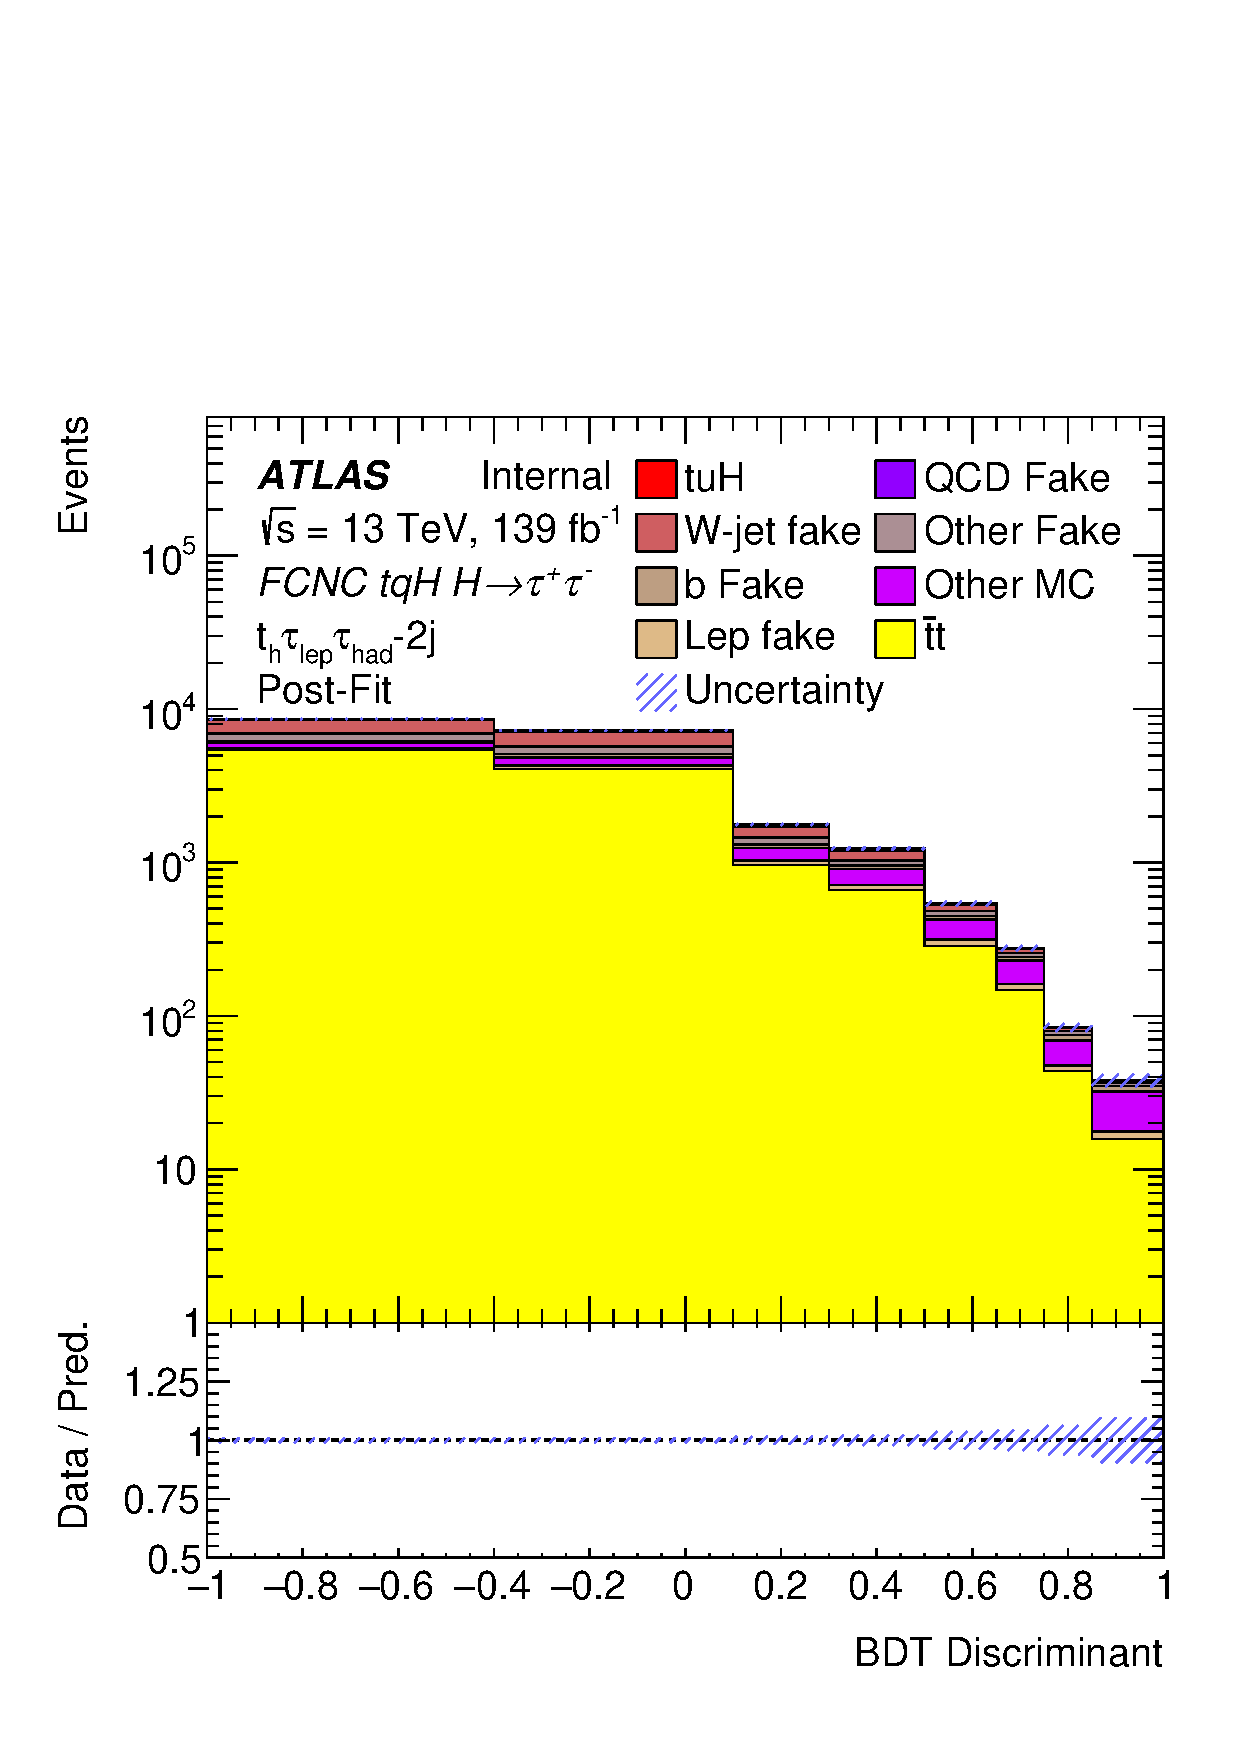
\includegraphics[width=0.30\textwidth]{\FCNCFigures/tthML/Limit/tuH_reg1l1tau1b2j_os_postFit_BOnly.pdf}
\put(-100, 55){\textbf{(a3)}}\\
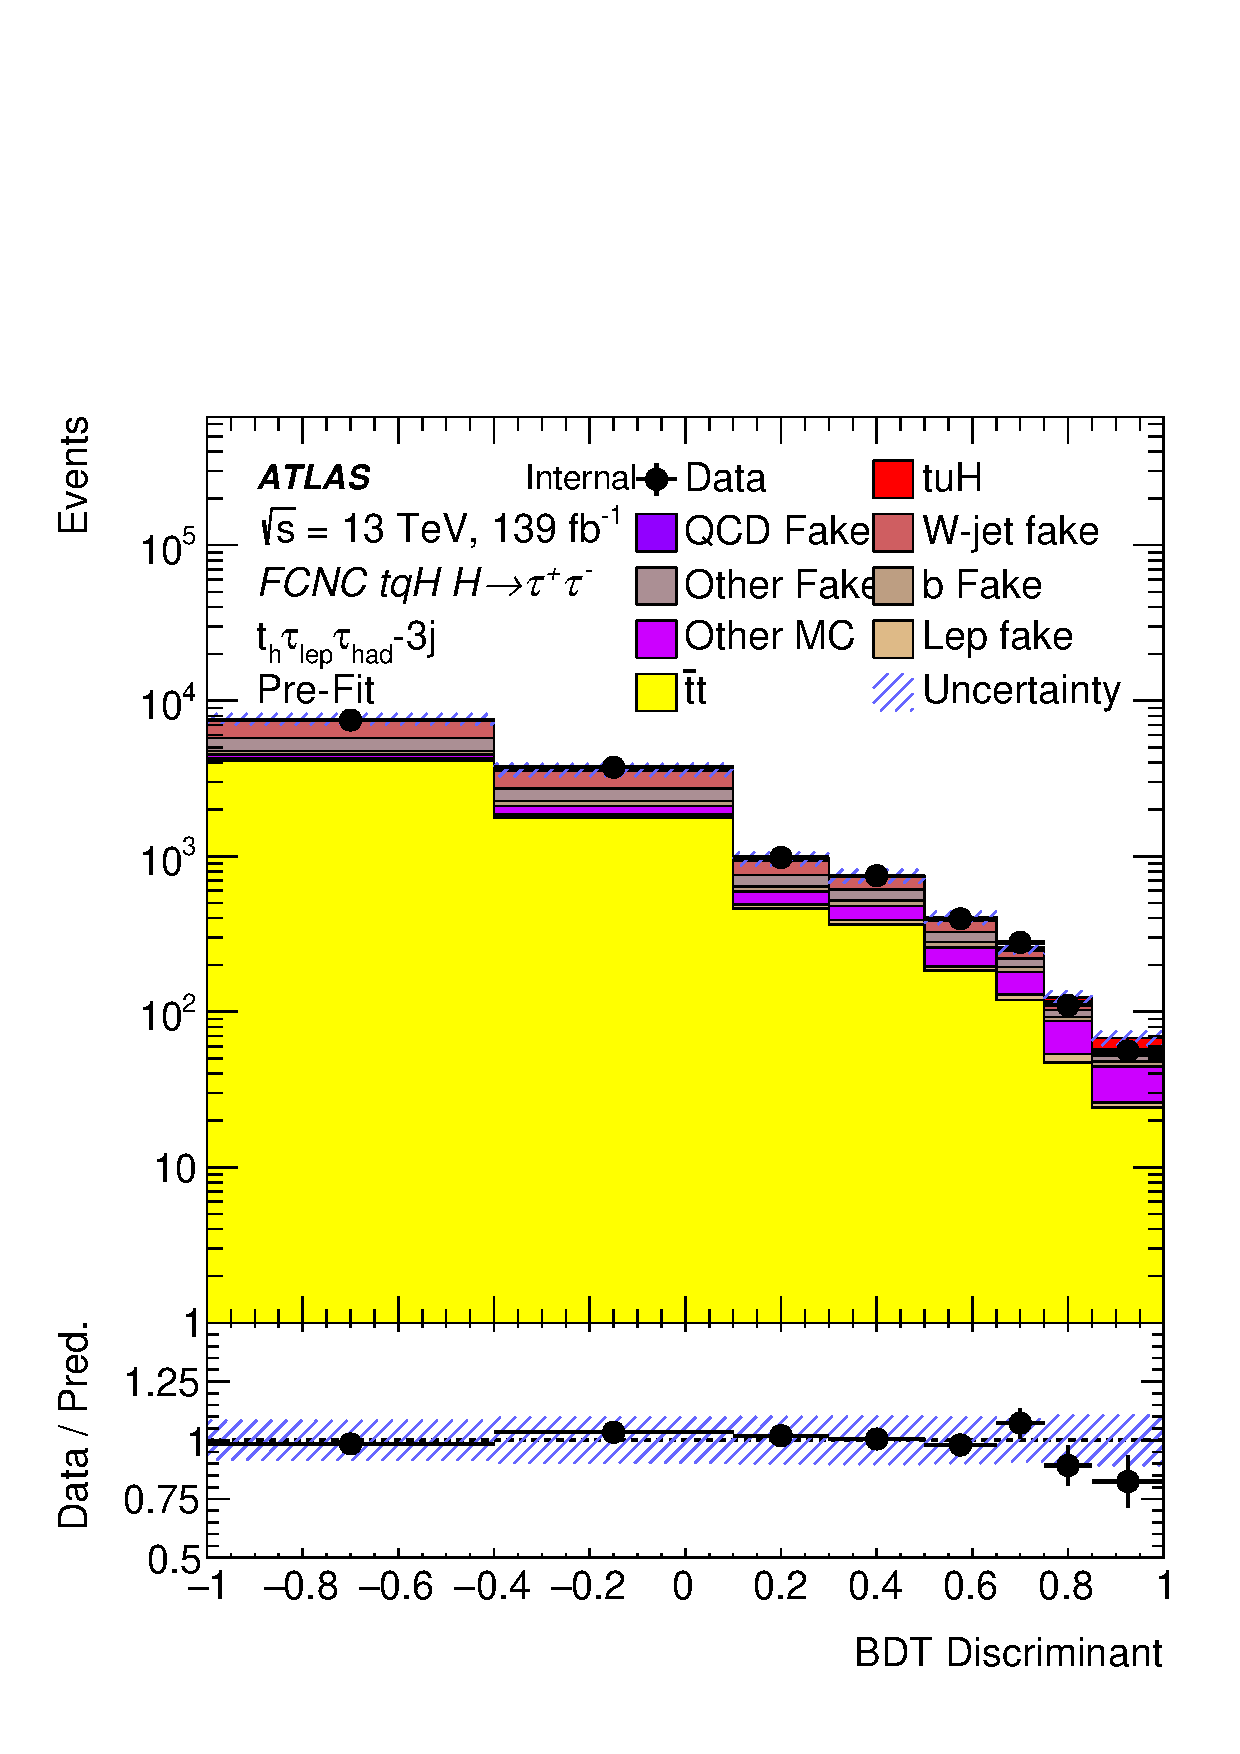
\includegraphics[width=0.30\textwidth]{\FCNCFigures/tthML/Limit/tuH_reg1l1tau1b3j_os.pdf}
\put(-100, 55){\textbf{(b1)}}
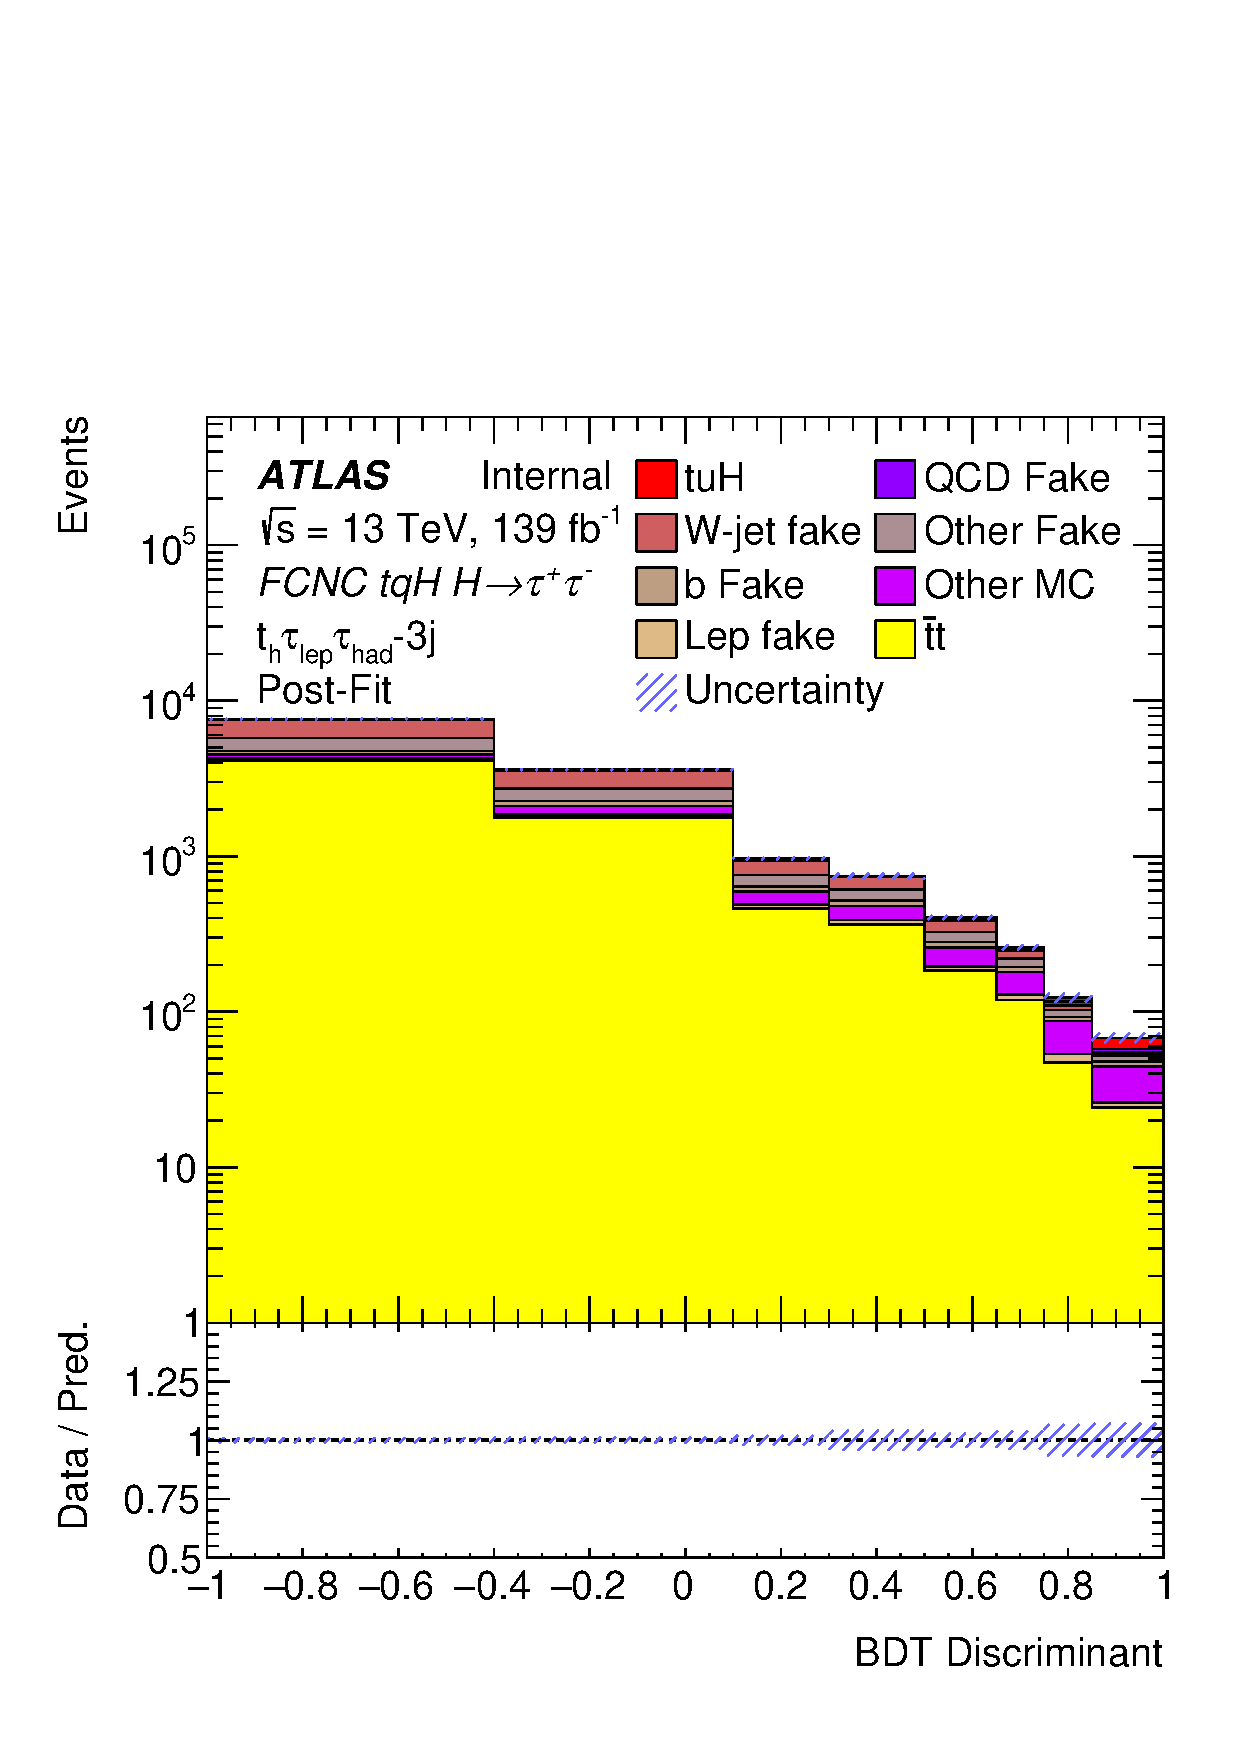
\includegraphics[width=0.30\textwidth]{\FCNCFigures/tthML/Limit/tuH_reg1l1tau1b3j_os_postFit.pdf}
\put(-100, 55){\textbf{(b2)}}
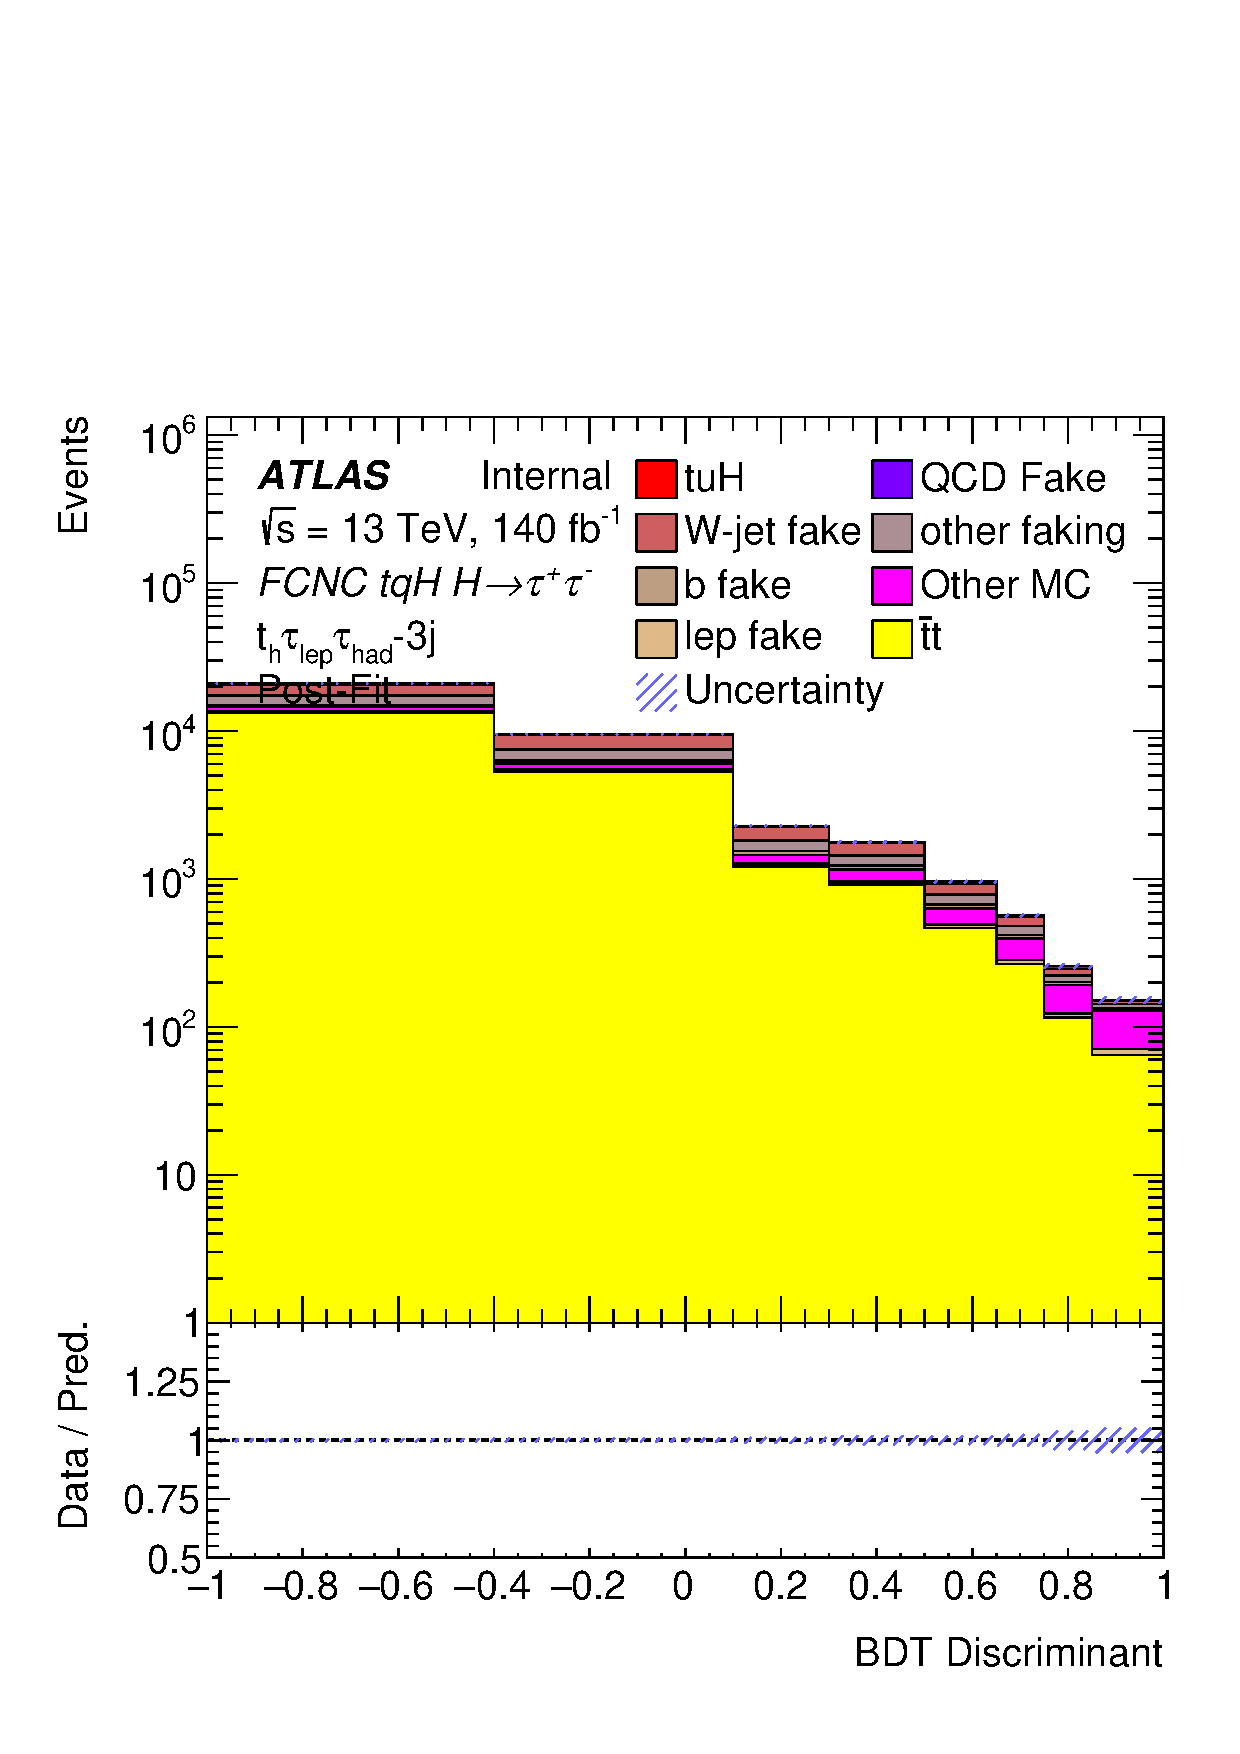
\includegraphics[width=0.30\textwidth]{\FCNCFigures/tthML/Limit/tuH_reg1l1tau1b3j_os_postFit_BOnly.pdf}
\put(-100, 55){\textbf{(b3)}}\\
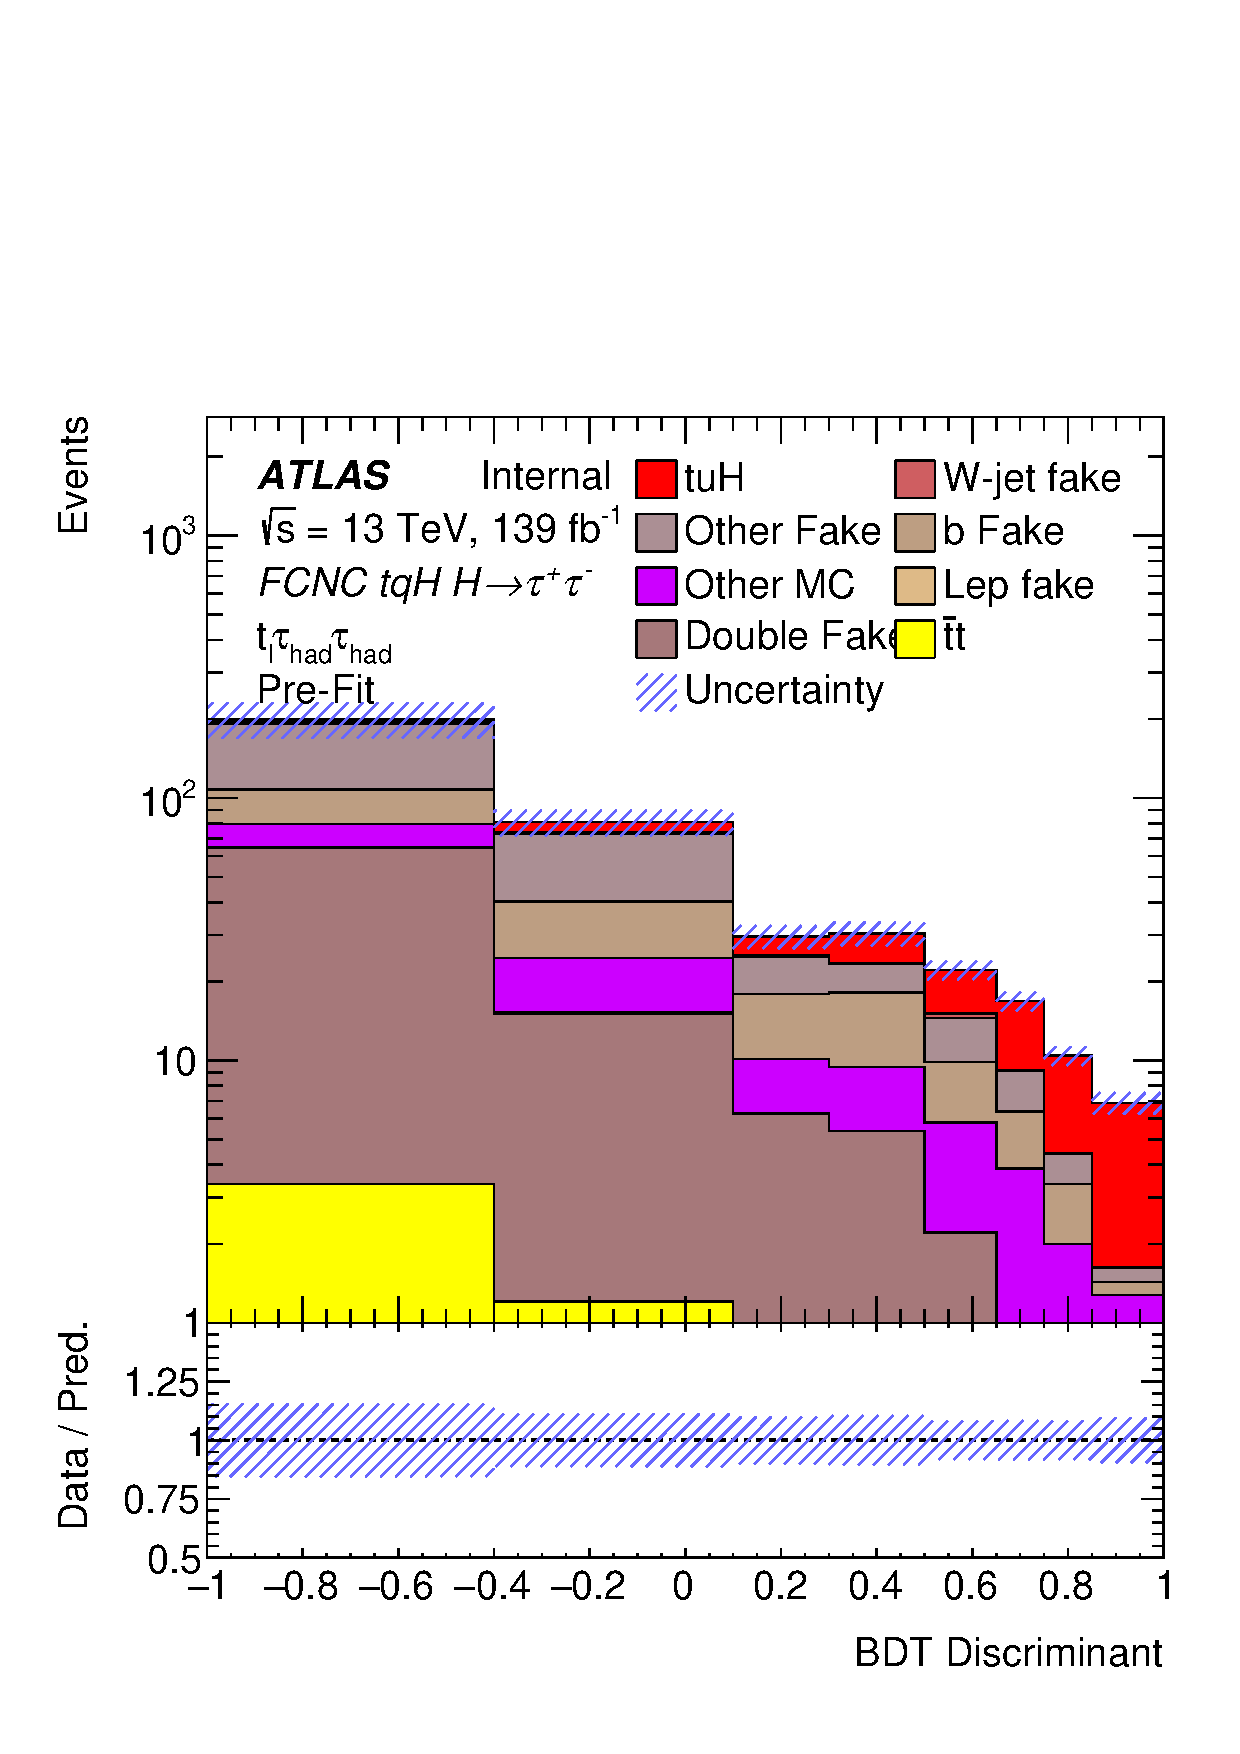
\includegraphics[width=0.30\textwidth]{\FCNCFigures/tthML/Limit/tuH_reg1l2tau1bnj_os.pdf}
\put(-100, 55){\textbf{(c1)}}
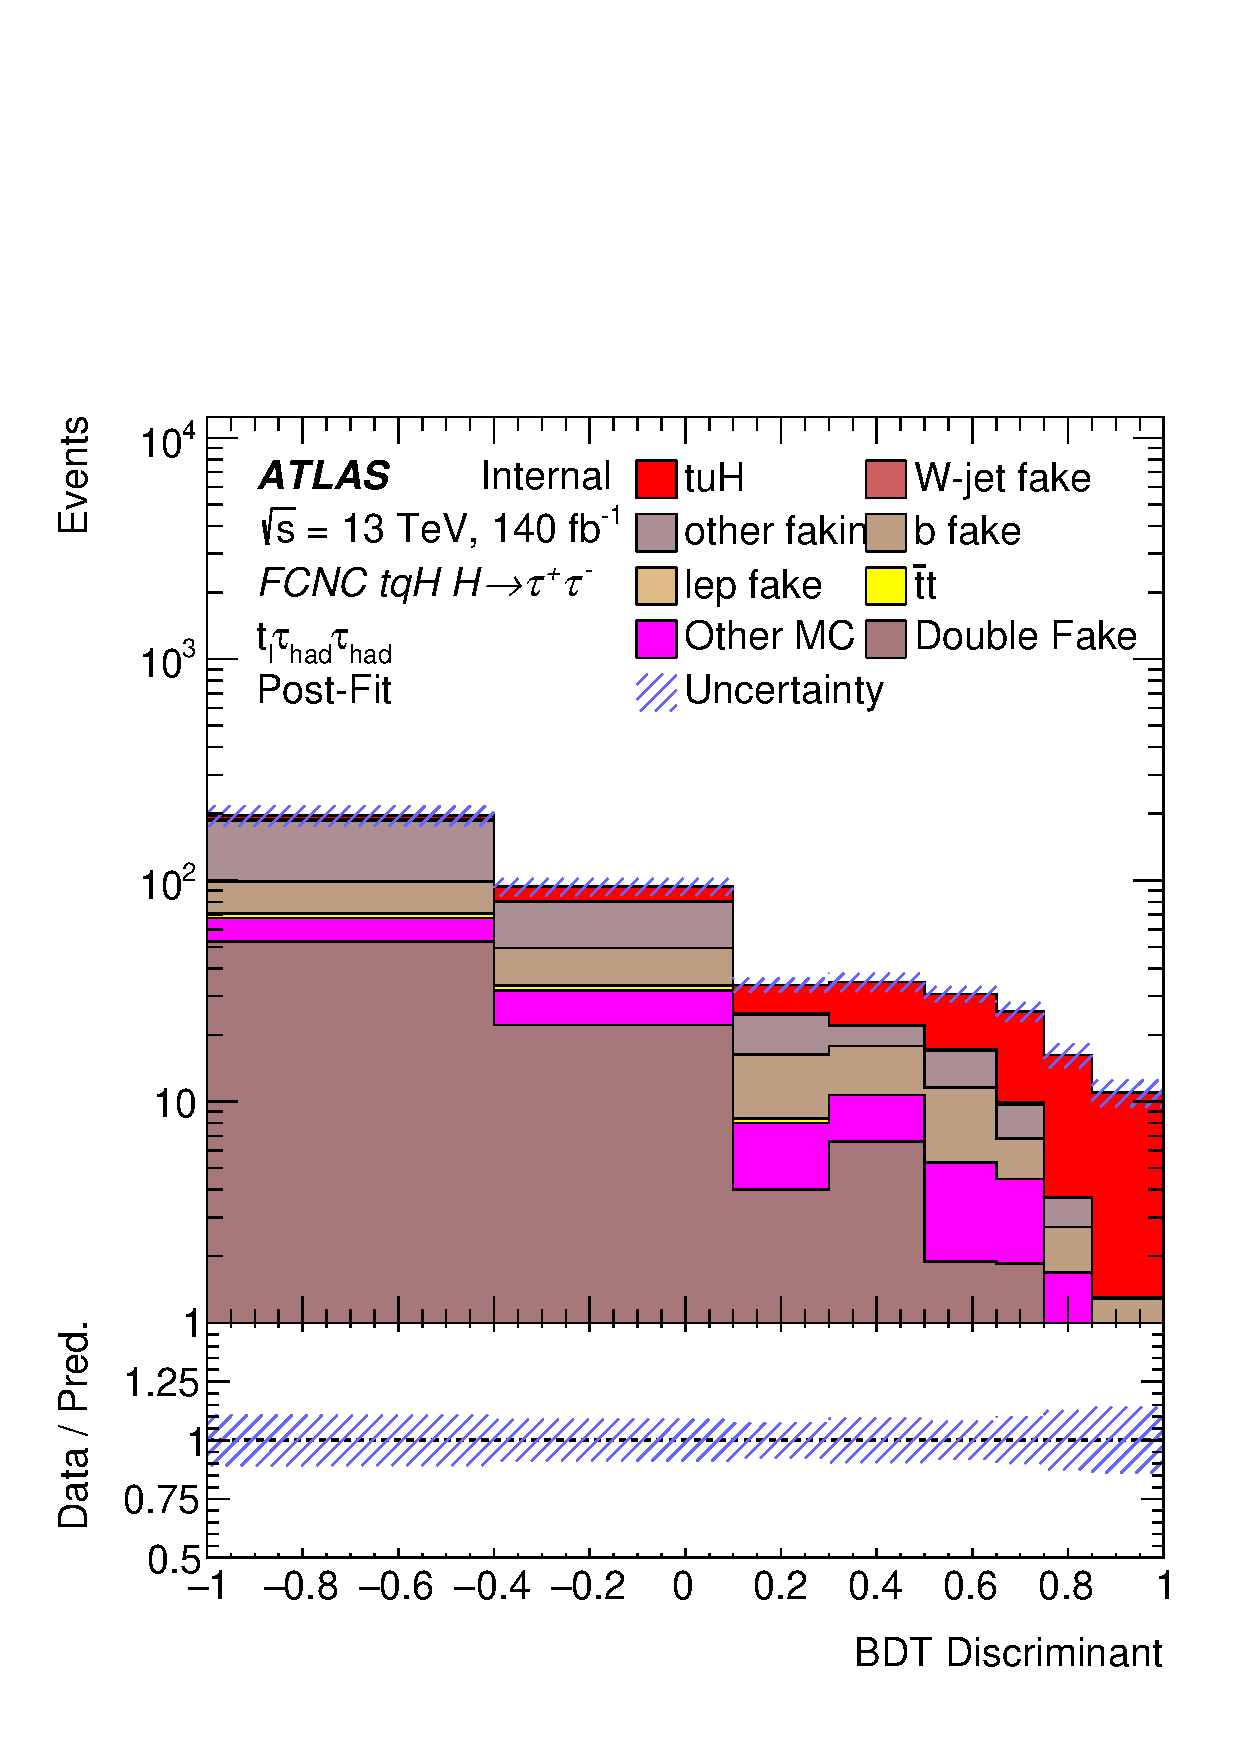
\includegraphics[width=0.30\textwidth]{\FCNCFigures/tthML/Limit/tuH_reg1l2tau1bnj_os_postFit.pdf}
\put(-100, 55){\textbf{(c2)}}
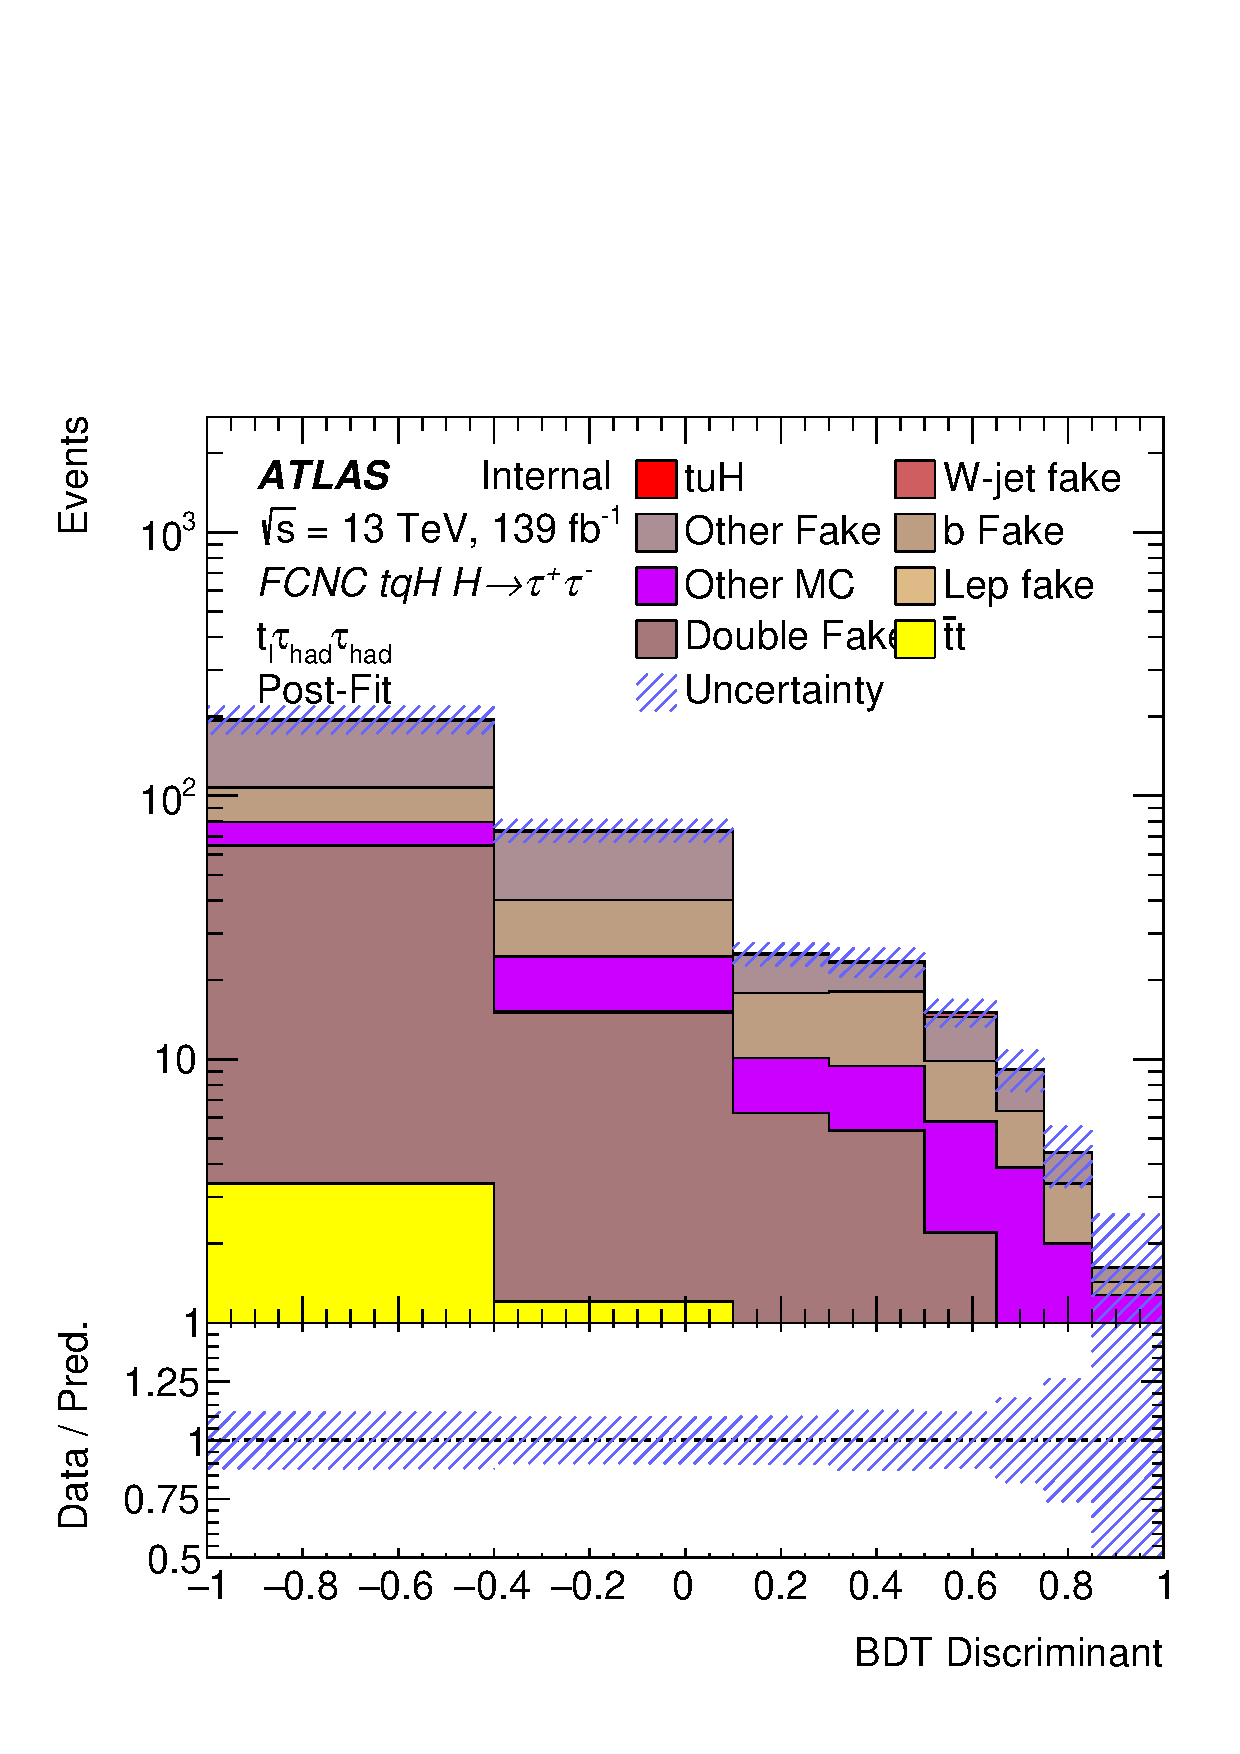
\includegraphics[width=0.30\textwidth]{\FCNCFigures/tthML/Limit/tuH_reg1l2tau1bnj_os_postFit_BOnly.pdf}
\put(-100, 55){\textbf{(c3)}}\\

\caption{ Comparison of the shape of the BDT discriminant distribution between the asimov prefit (a1,b1,c1), asimov postfit  with $\mu$=1 (a2,b2,c2) and background only fit (a3,b3,c3) in terms of tuH merged signal. The upper three plots are in the  $t_h\tlhad$-2j (a1-a3) region, the medium three are in $t_h\tlhad$-3j (b1-b3) and the bottom three are in $t_l\thadhad$ (c1-c3) . Statistical and systematic uncertainties are being shown.}
\label{fig:tthML_trexPrefit}
\end{figure}

\begin{figure}[H]
\centering
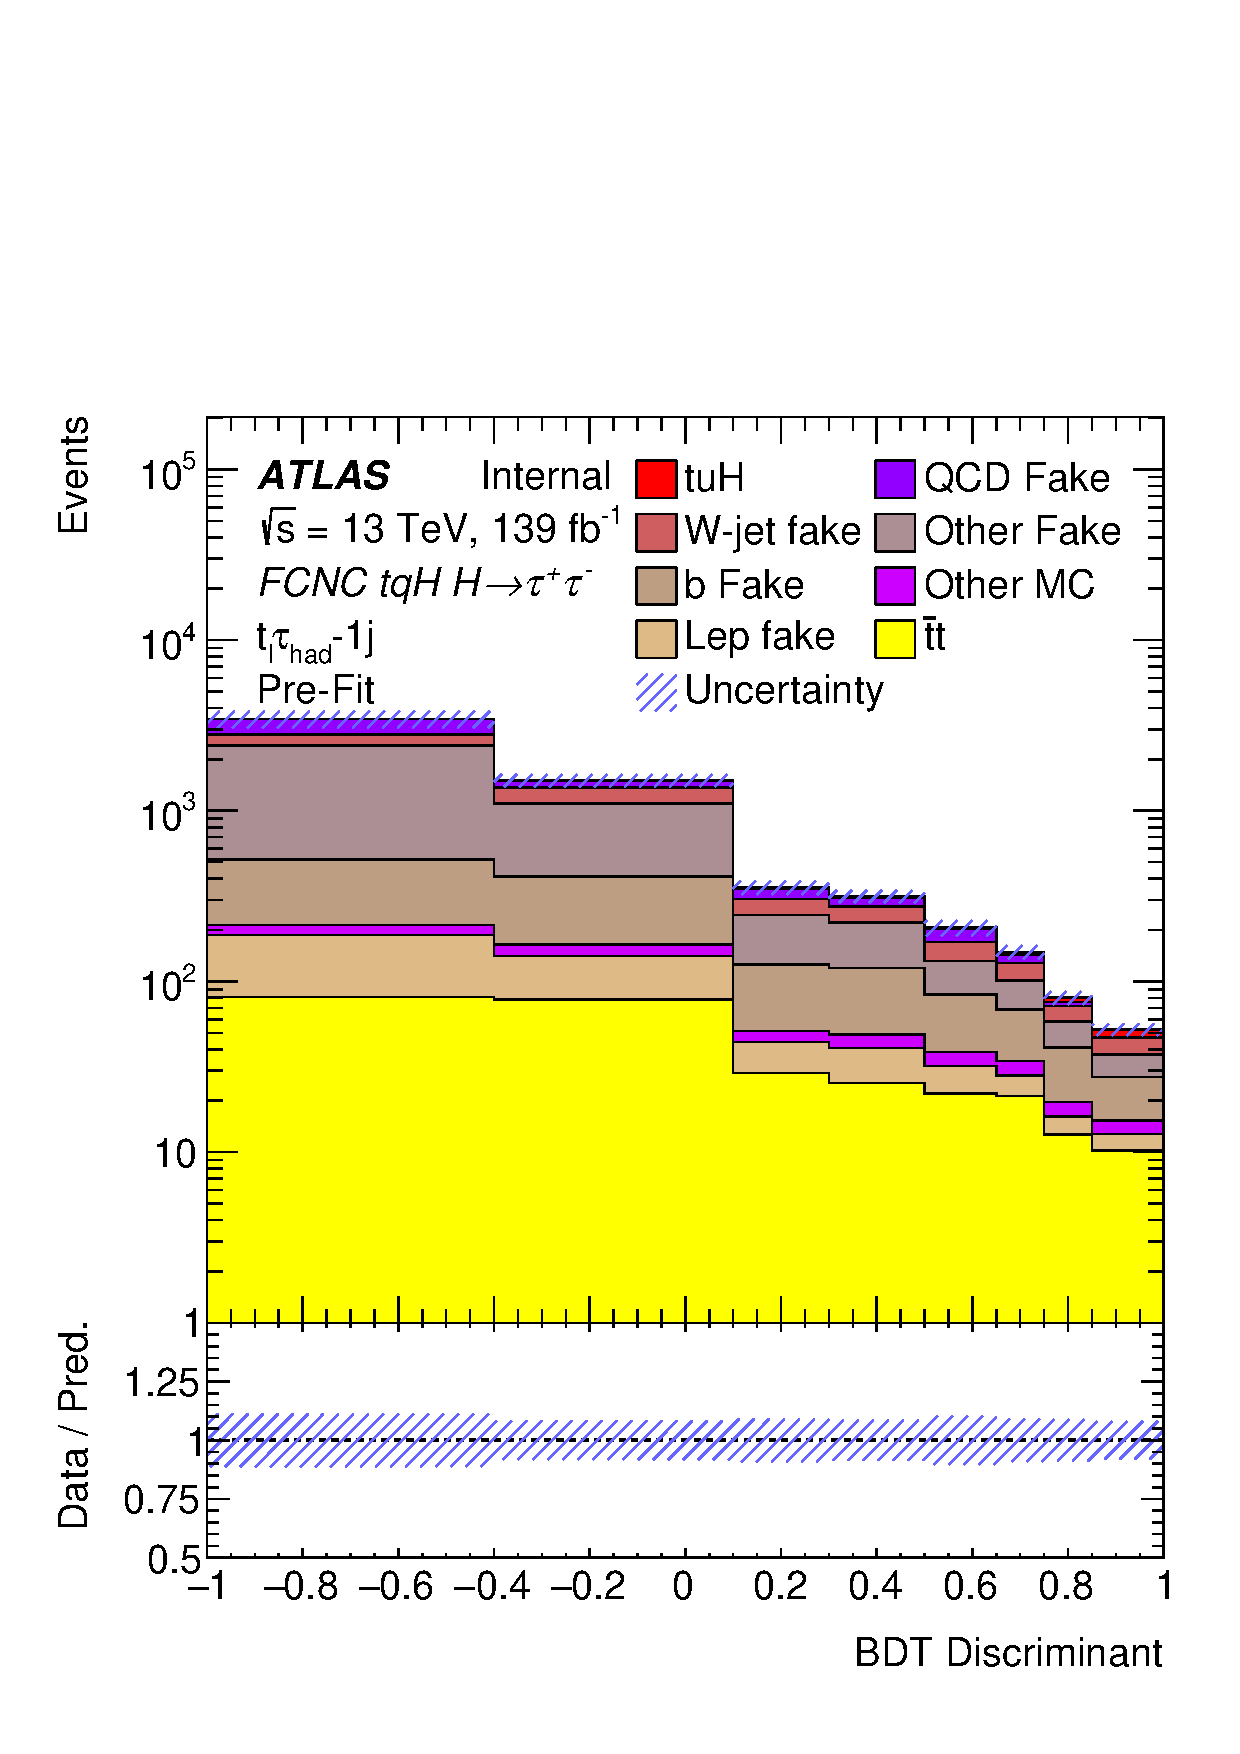
\includegraphics[width=0.30\textwidth]{\FCNCFigures/tthML/Limit/tuH_reg1l1tau1b1j_ss.pdf}
\put(-100, 55){\textbf{(a1)}}
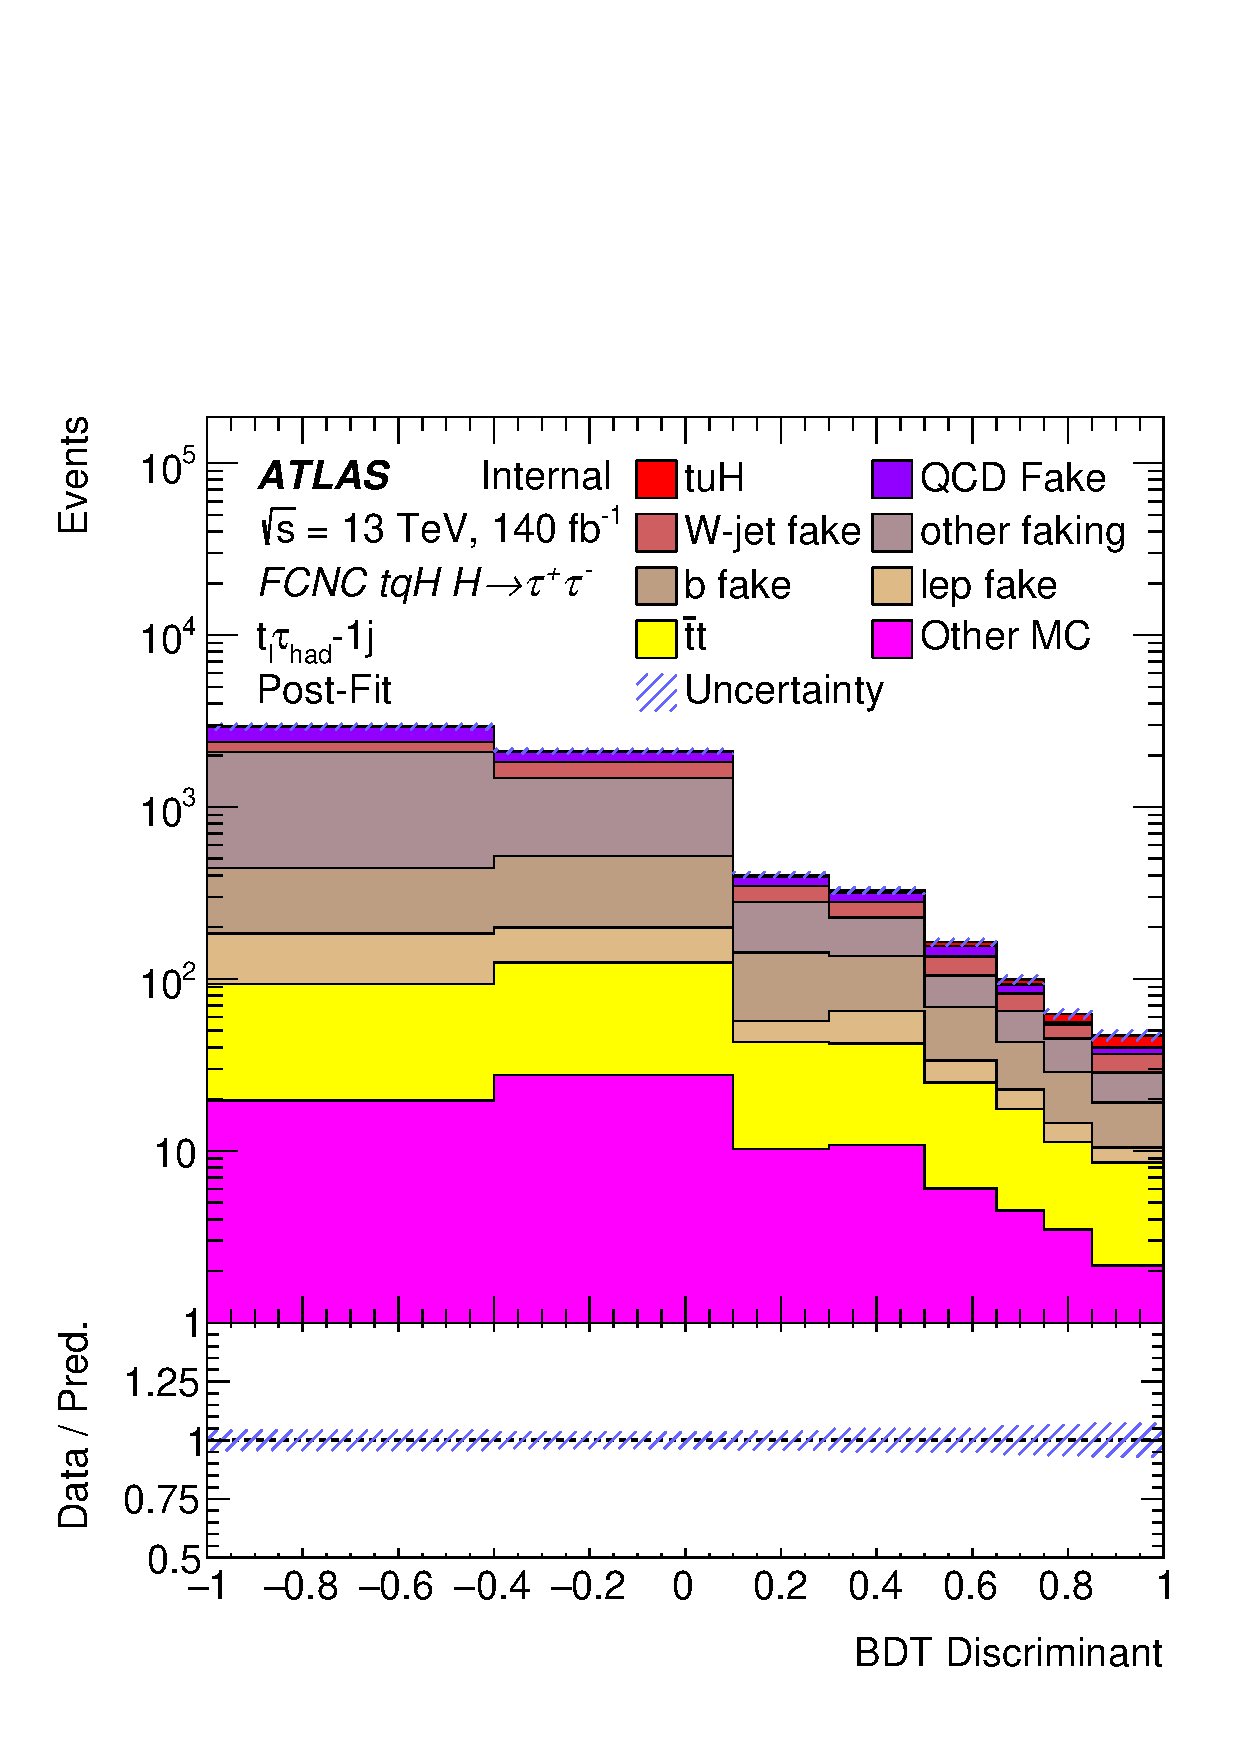
\includegraphics[width=0.30\textwidth]{\FCNCFigures/tthML/Limit/tuH_reg1l1tau1b1j_ss_postFit.pdf}
\put(-100, 55){\textbf{(a2)}}
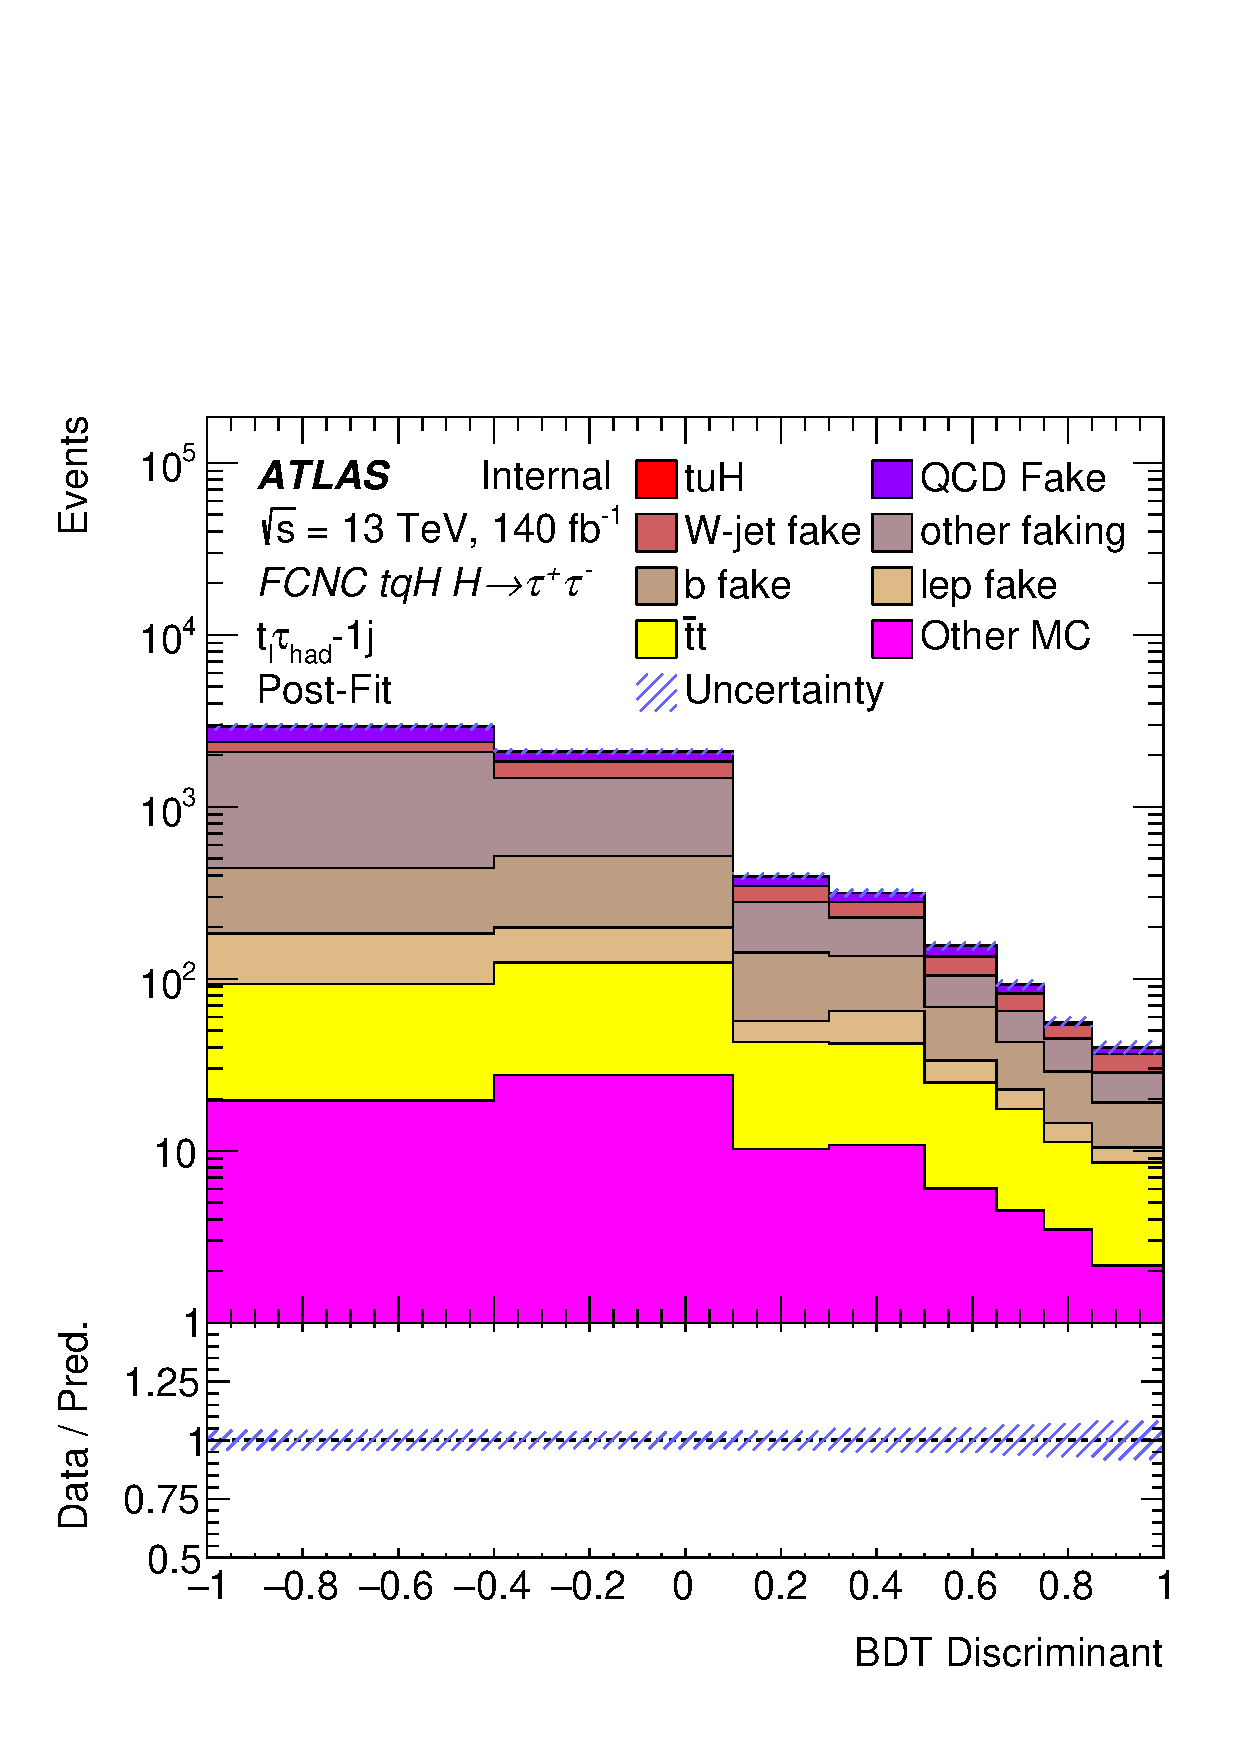
\includegraphics[width=0.30\textwidth]{\FCNCFigures/tthML/Limit/tuH_reg1l1tau1b1j_ss_postFit_BOnly.pdf}
\put(-100, 55){\textbf{(a3)}}\\
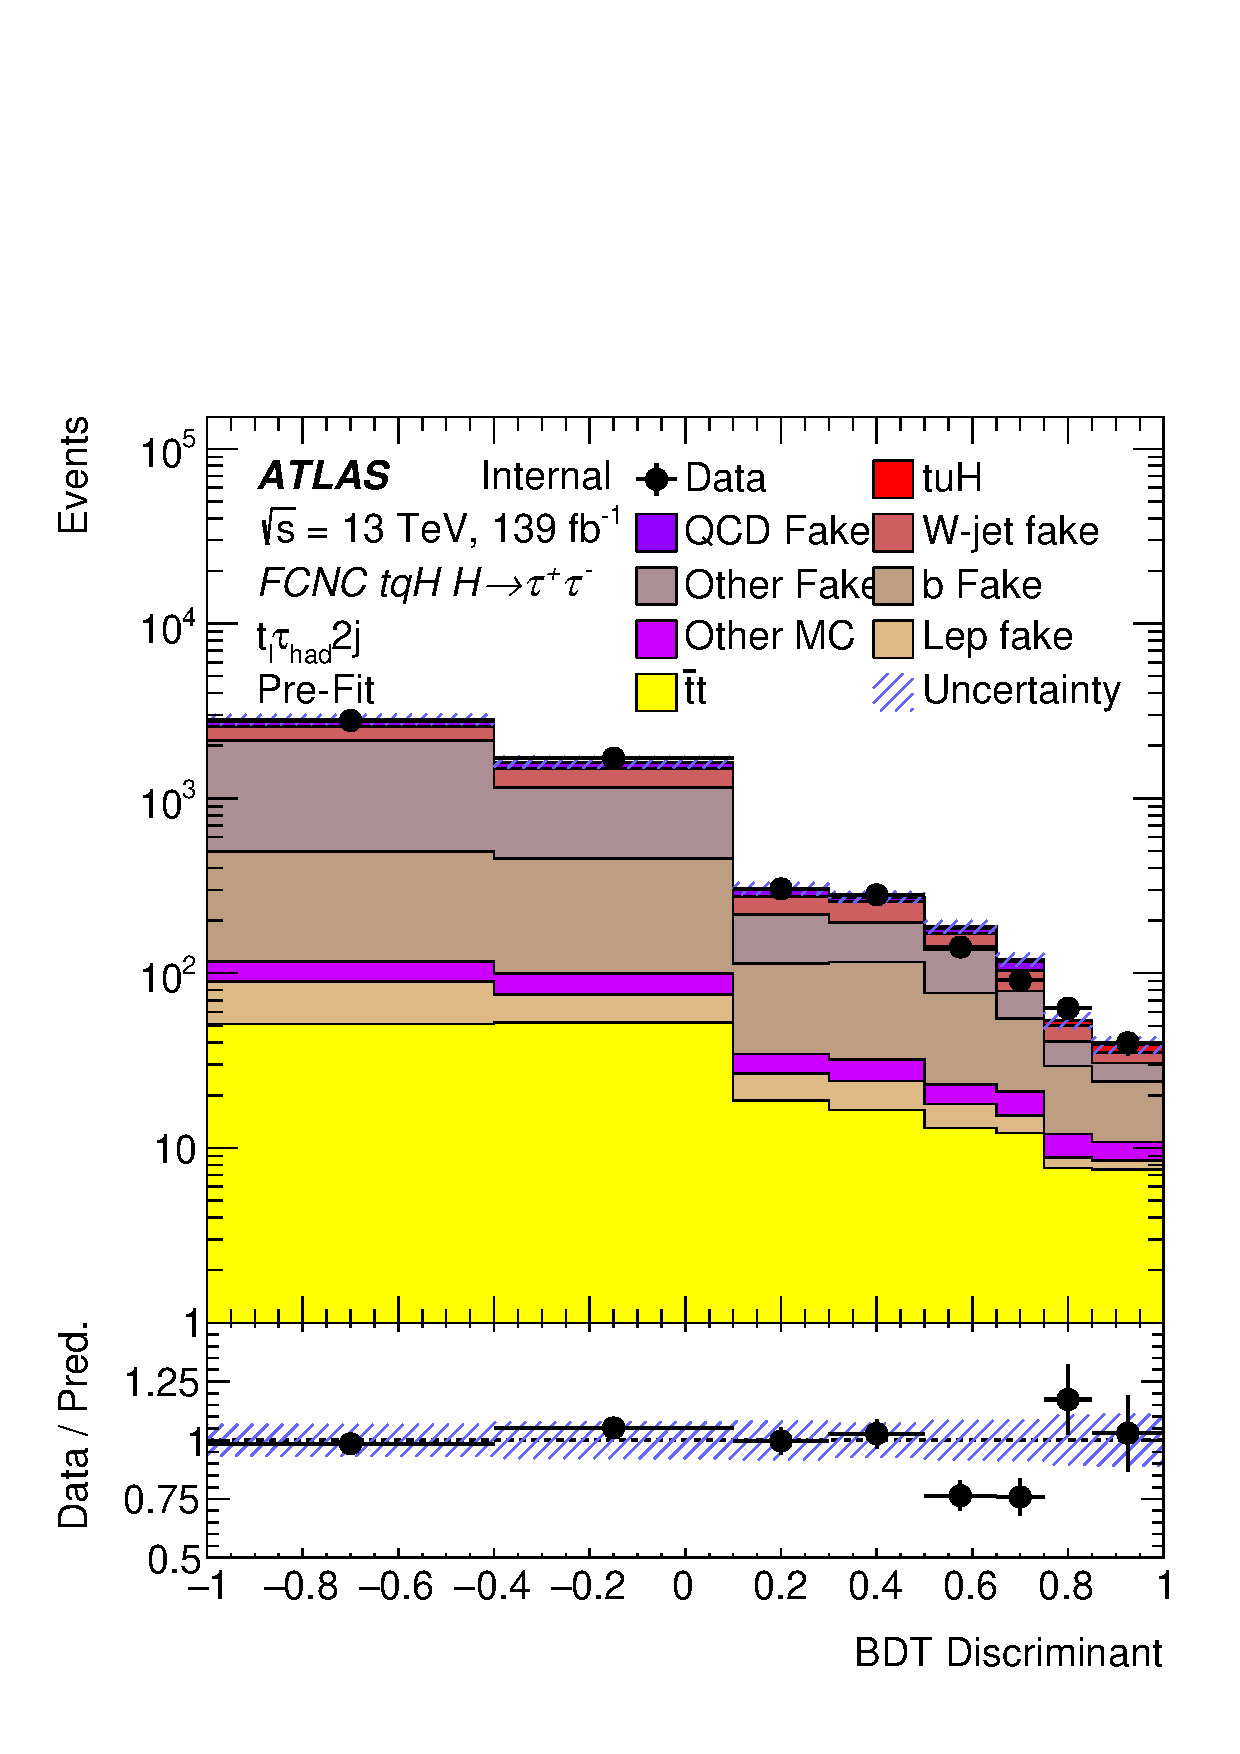
\includegraphics[width=0.30\textwidth]{\FCNCFigures/tthML/Limit/tuH_reg1l1tau1b2j_ss.pdf}
\put(-100, 55){\textbf{(b1)}}
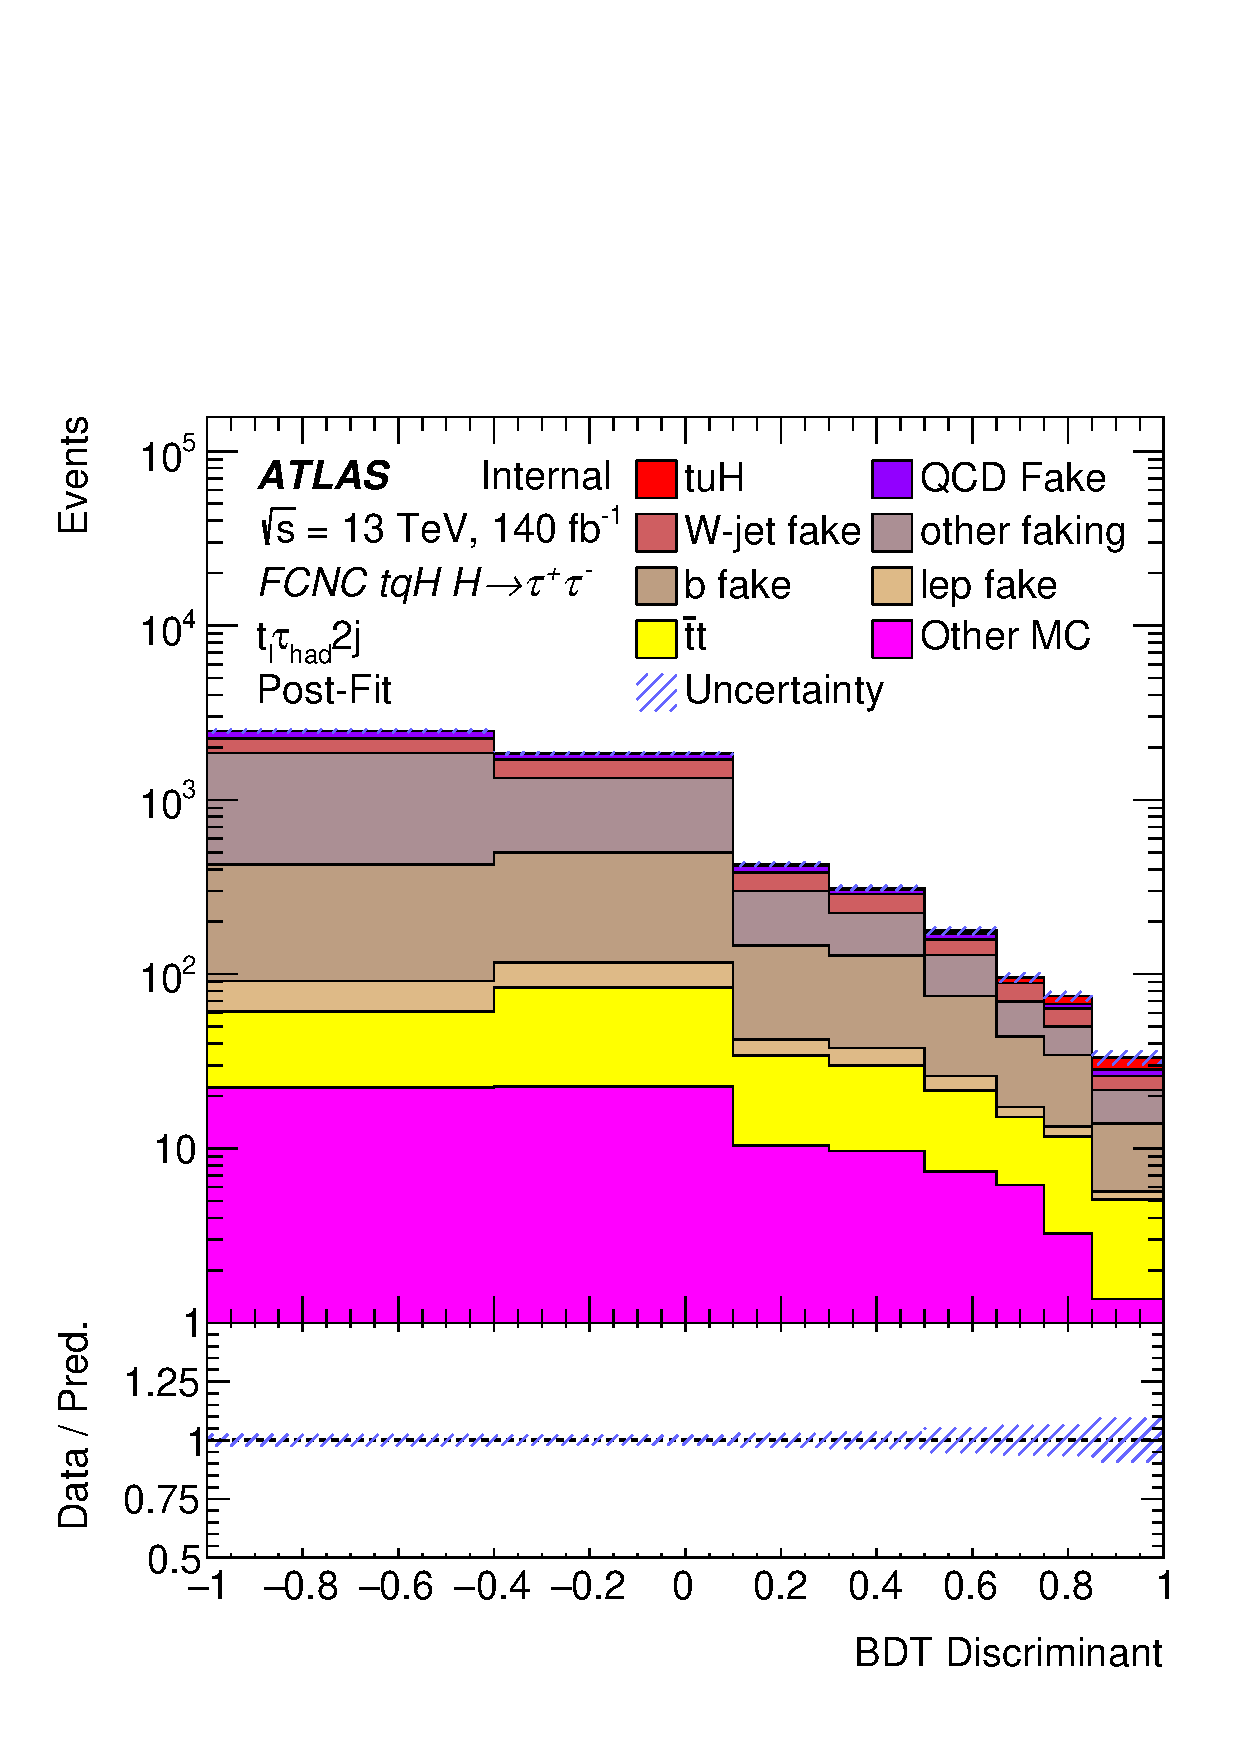
\includegraphics[width=0.30\textwidth]{\FCNCFigures/tthML/Limit/tuH_reg1l1tau1b2j_ss_postFit.pdf}
\put(-100, 55){\textbf{(b2)}}
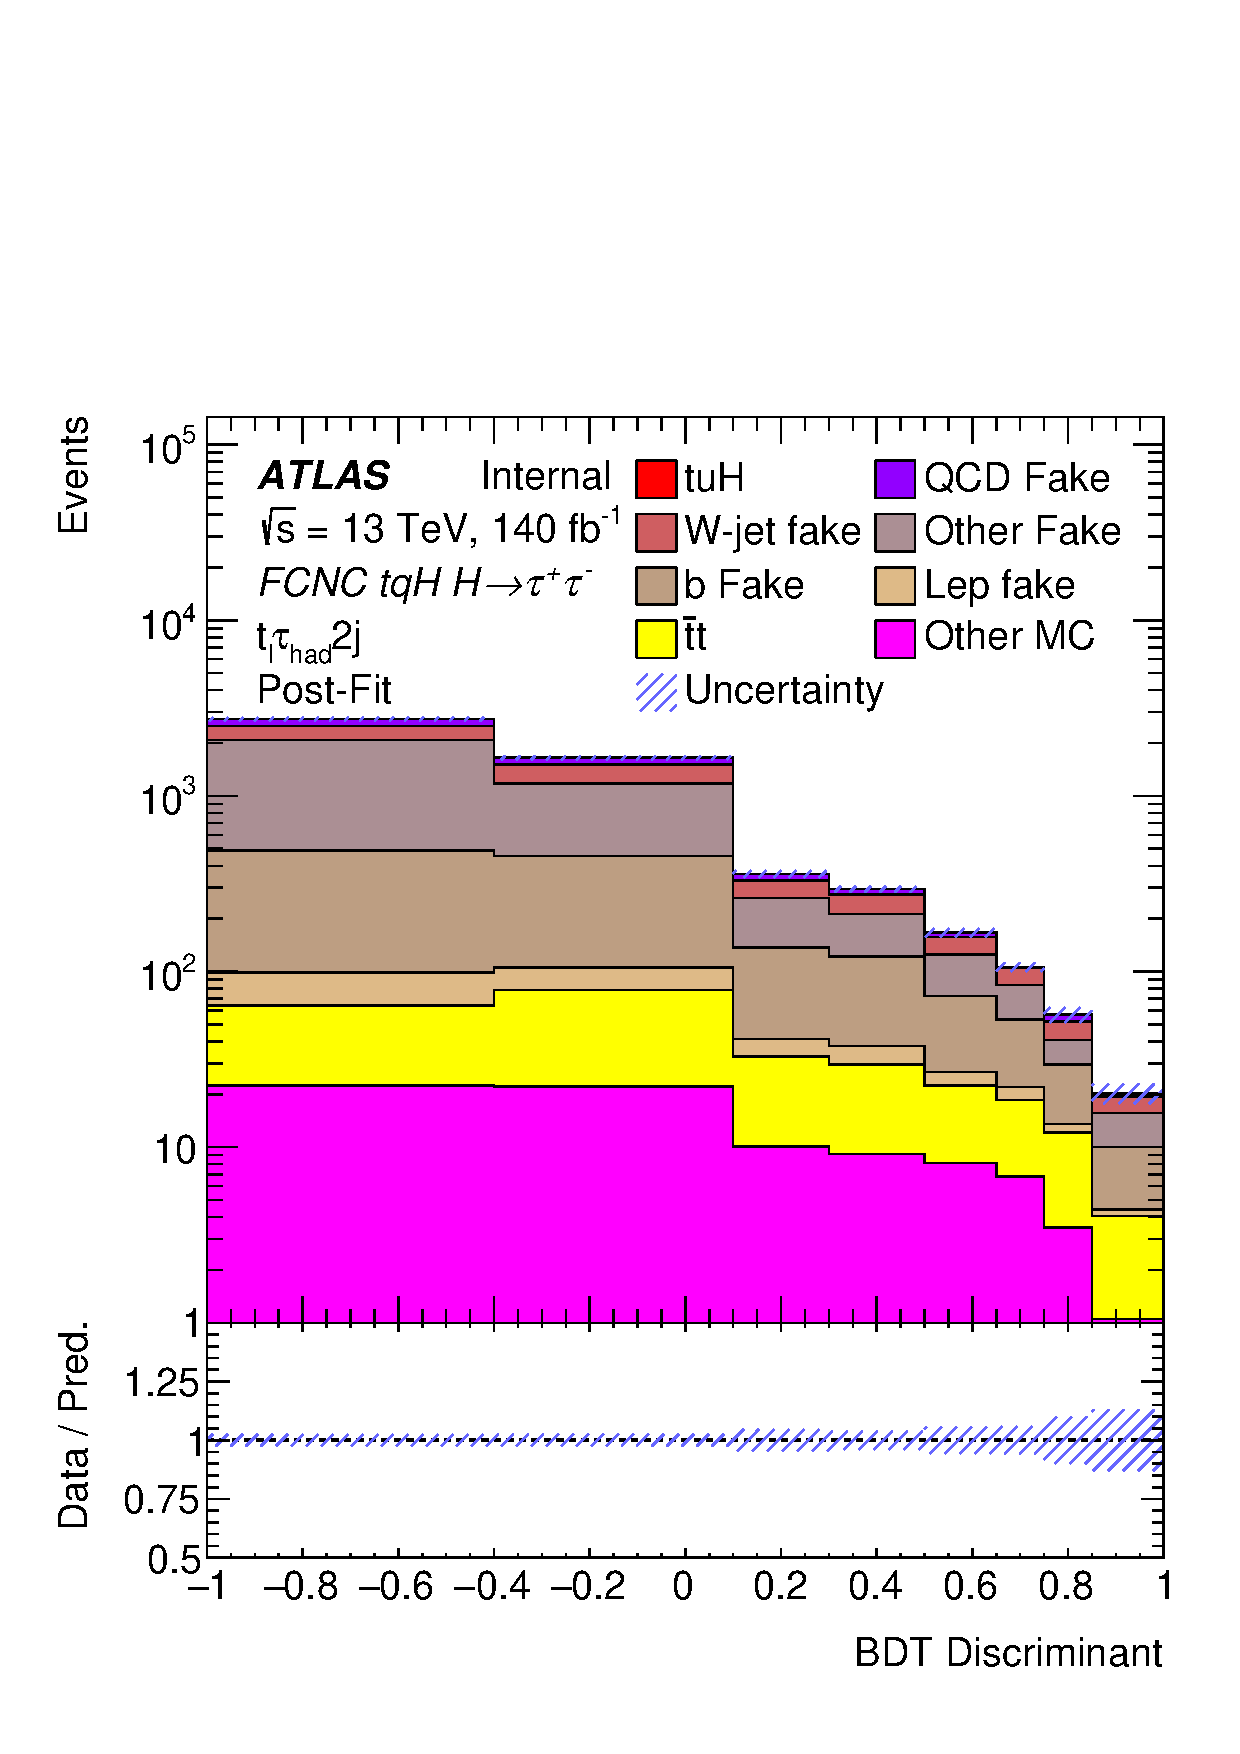
\includegraphics[width=0.30\textwidth]{\FCNCFigures/tthML/Limit/tuH_reg1l1tau1b2j_ss_postFit_BOnly.pdf}
\put(-100, 55){\textbf{(b3)}}\\

\caption{ Comparison of the shape of the BDT discriminant distribution between the asimov prefit (a1,b1), asimov postfit  with $\mu$=1 (a2,b2) and background only fit(a3,b3) in terms of tuH merged signal.The upper three plots are in the  $t_l\tauhad$-1j (a1-a3) region, and the bottom three are in $t_l\tauhad$-2j (b1-b3).Statistical and systematic uncertainties are being shown.}
\label{fig:tthML_trexPrefit_1}
\end{figure}

\begin{figure}[H]
\centering
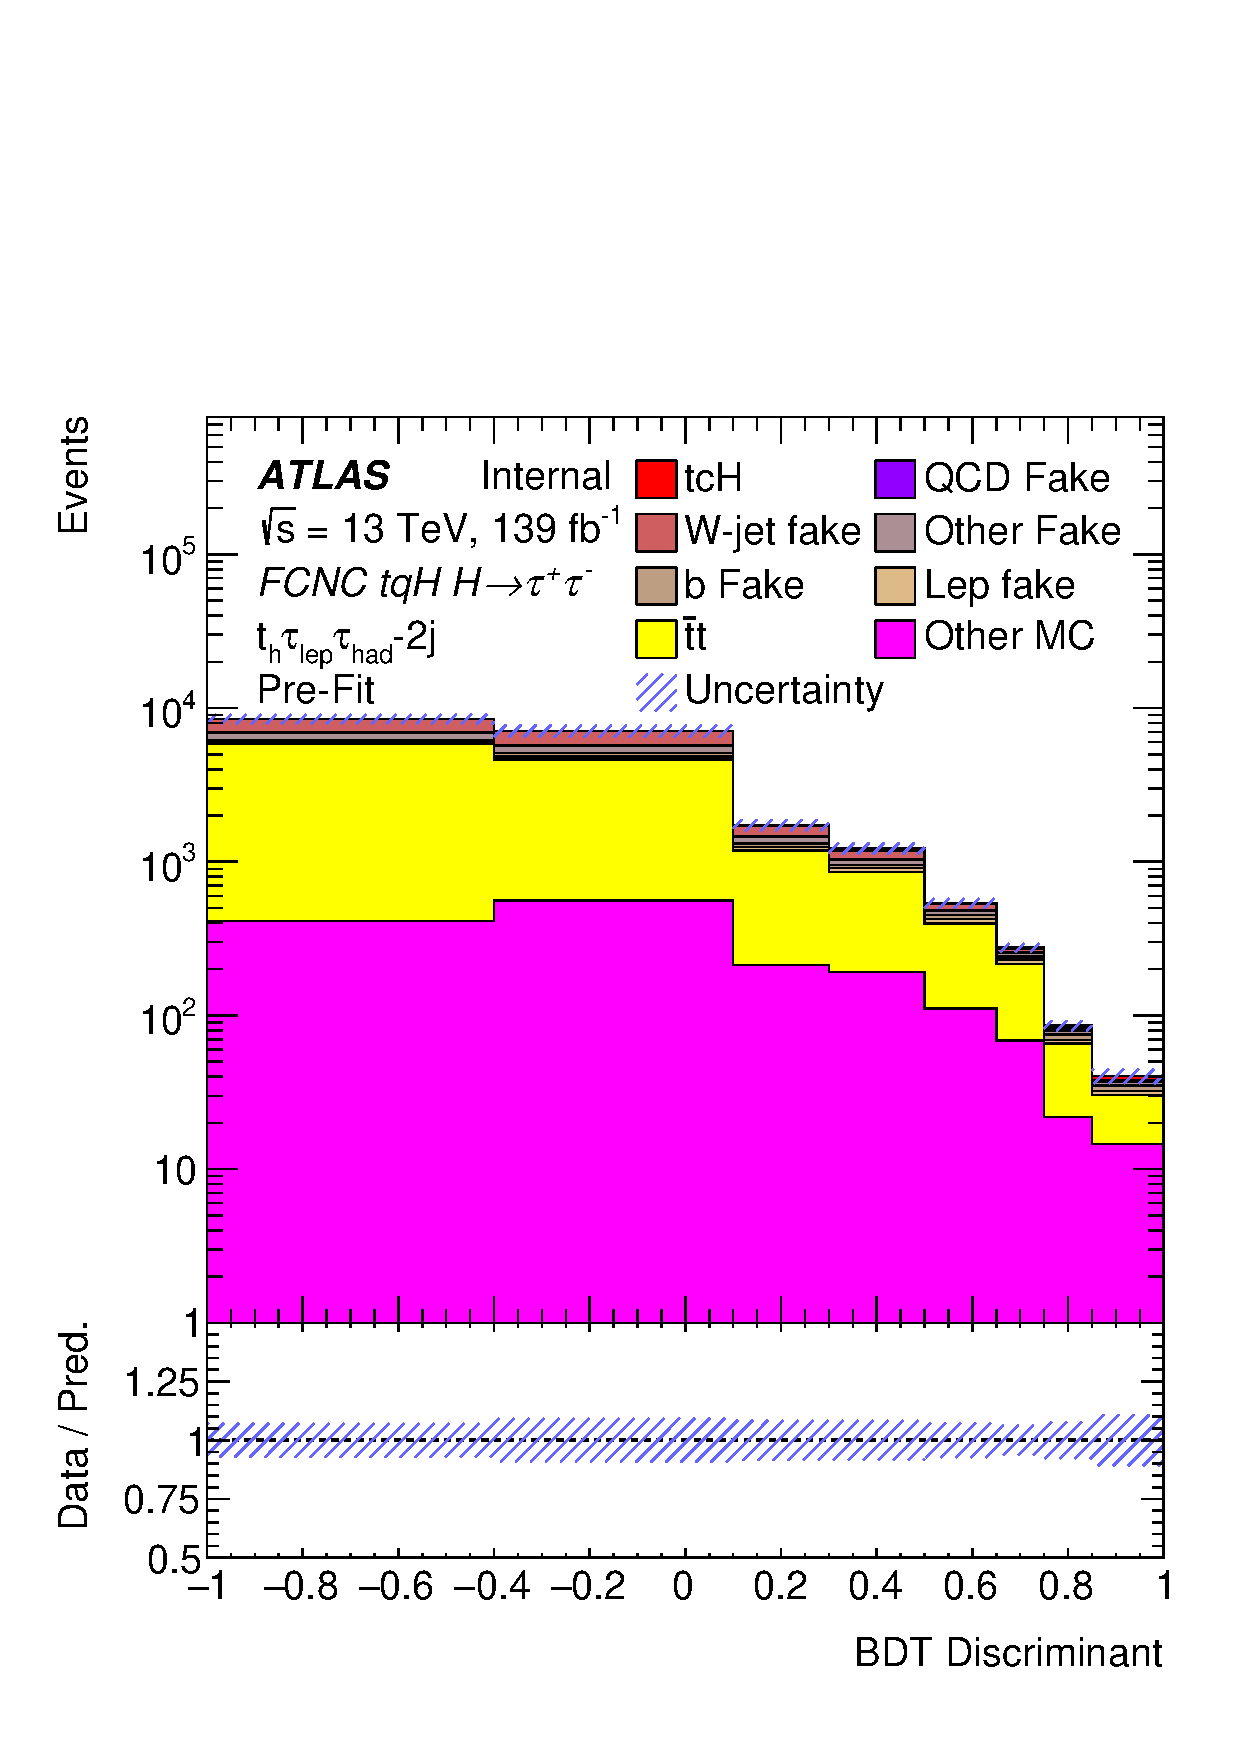
\includegraphics[width=0.30\textwidth]{\FCNCFigures/tthML/Limit/tcH_reg1l1tau1b2j_os.pdf}
\put(-100, 55){\textbf{(a1)}}
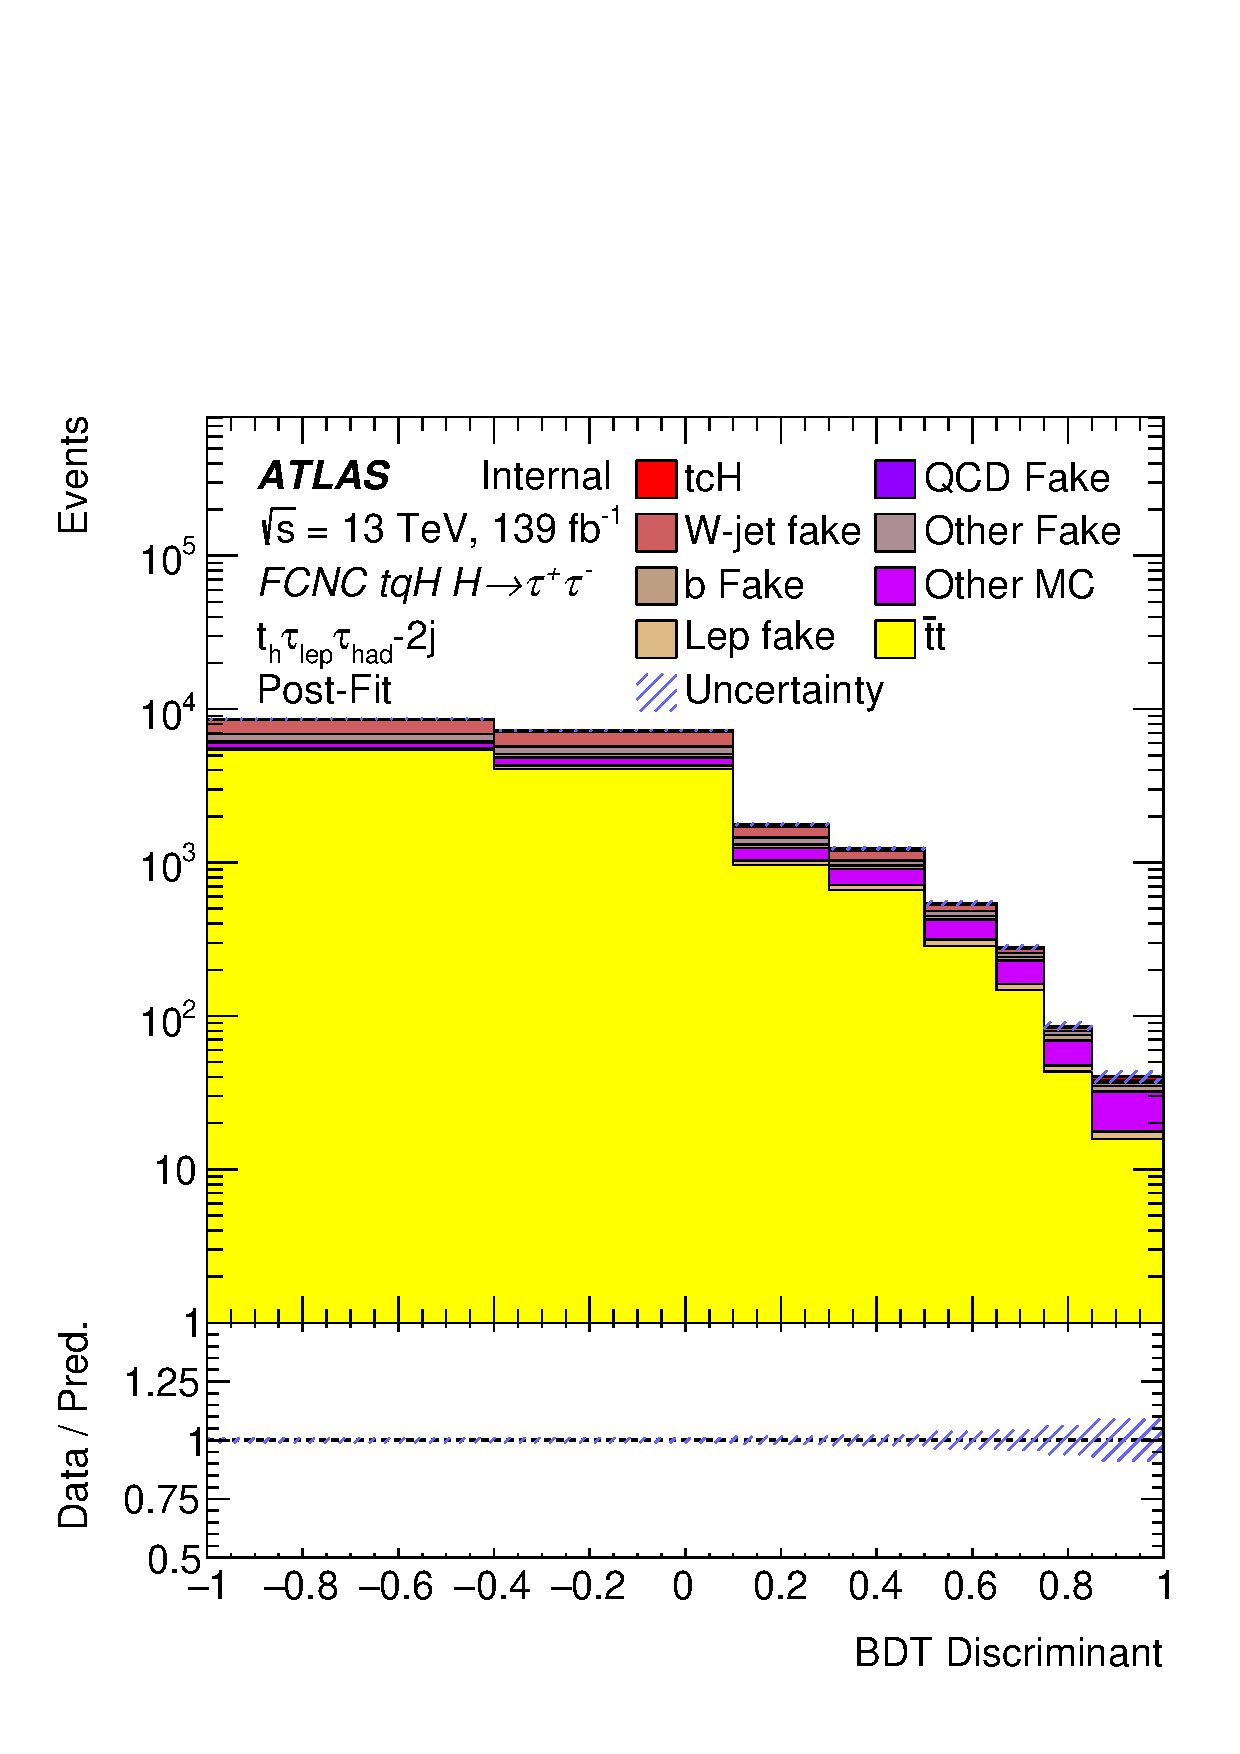
\includegraphics[width=0.30\textwidth]{\FCNCFigures/tthML/Limit/tcH_reg1l1tau1b2j_os_postFit.pdf}
\put(-100, 55){\textbf{(a2)}}
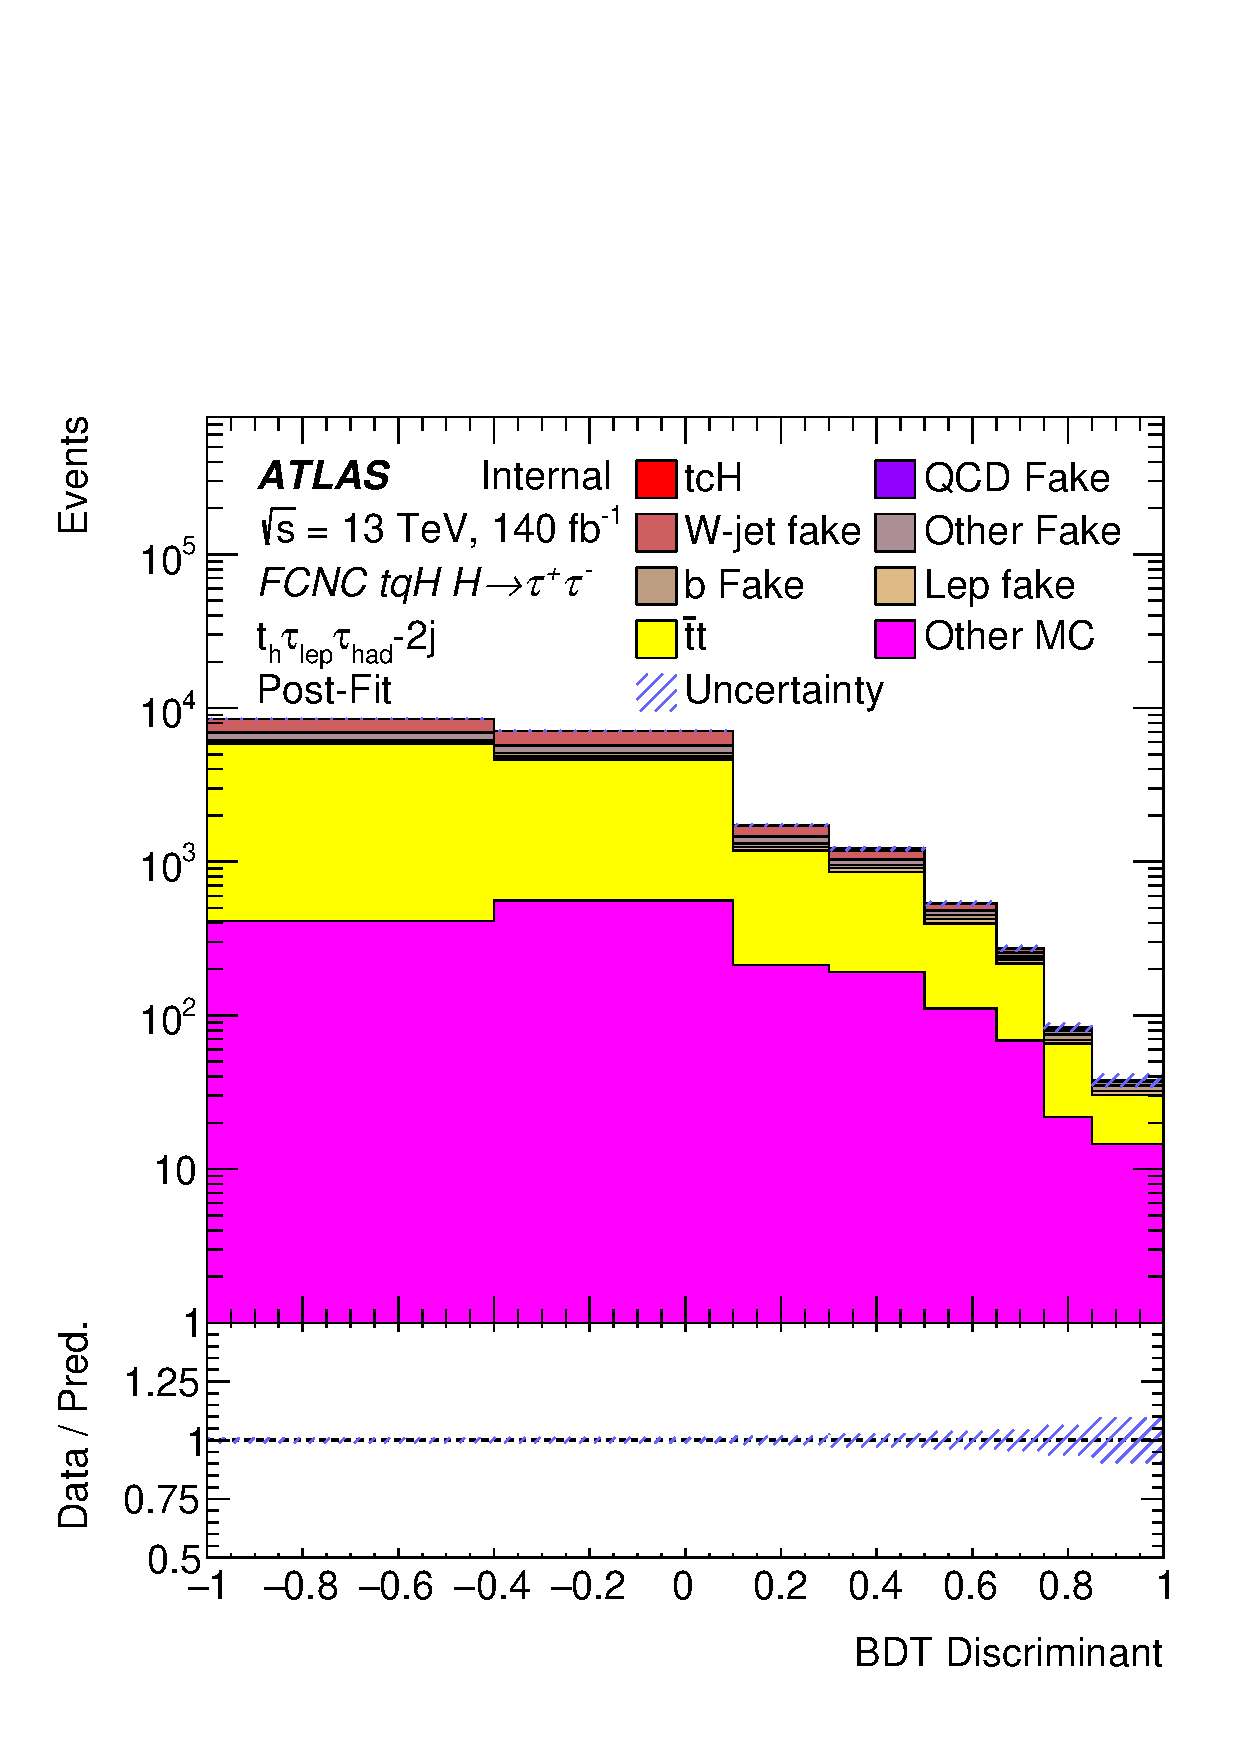
\includegraphics[width=0.30\textwidth]{\FCNCFigures/tthML/Limit/tcH_reg1l1tau1b2j_os_postFit_BOnly.pdf}
\put(-100, 55){\textbf{(a3)}}\\
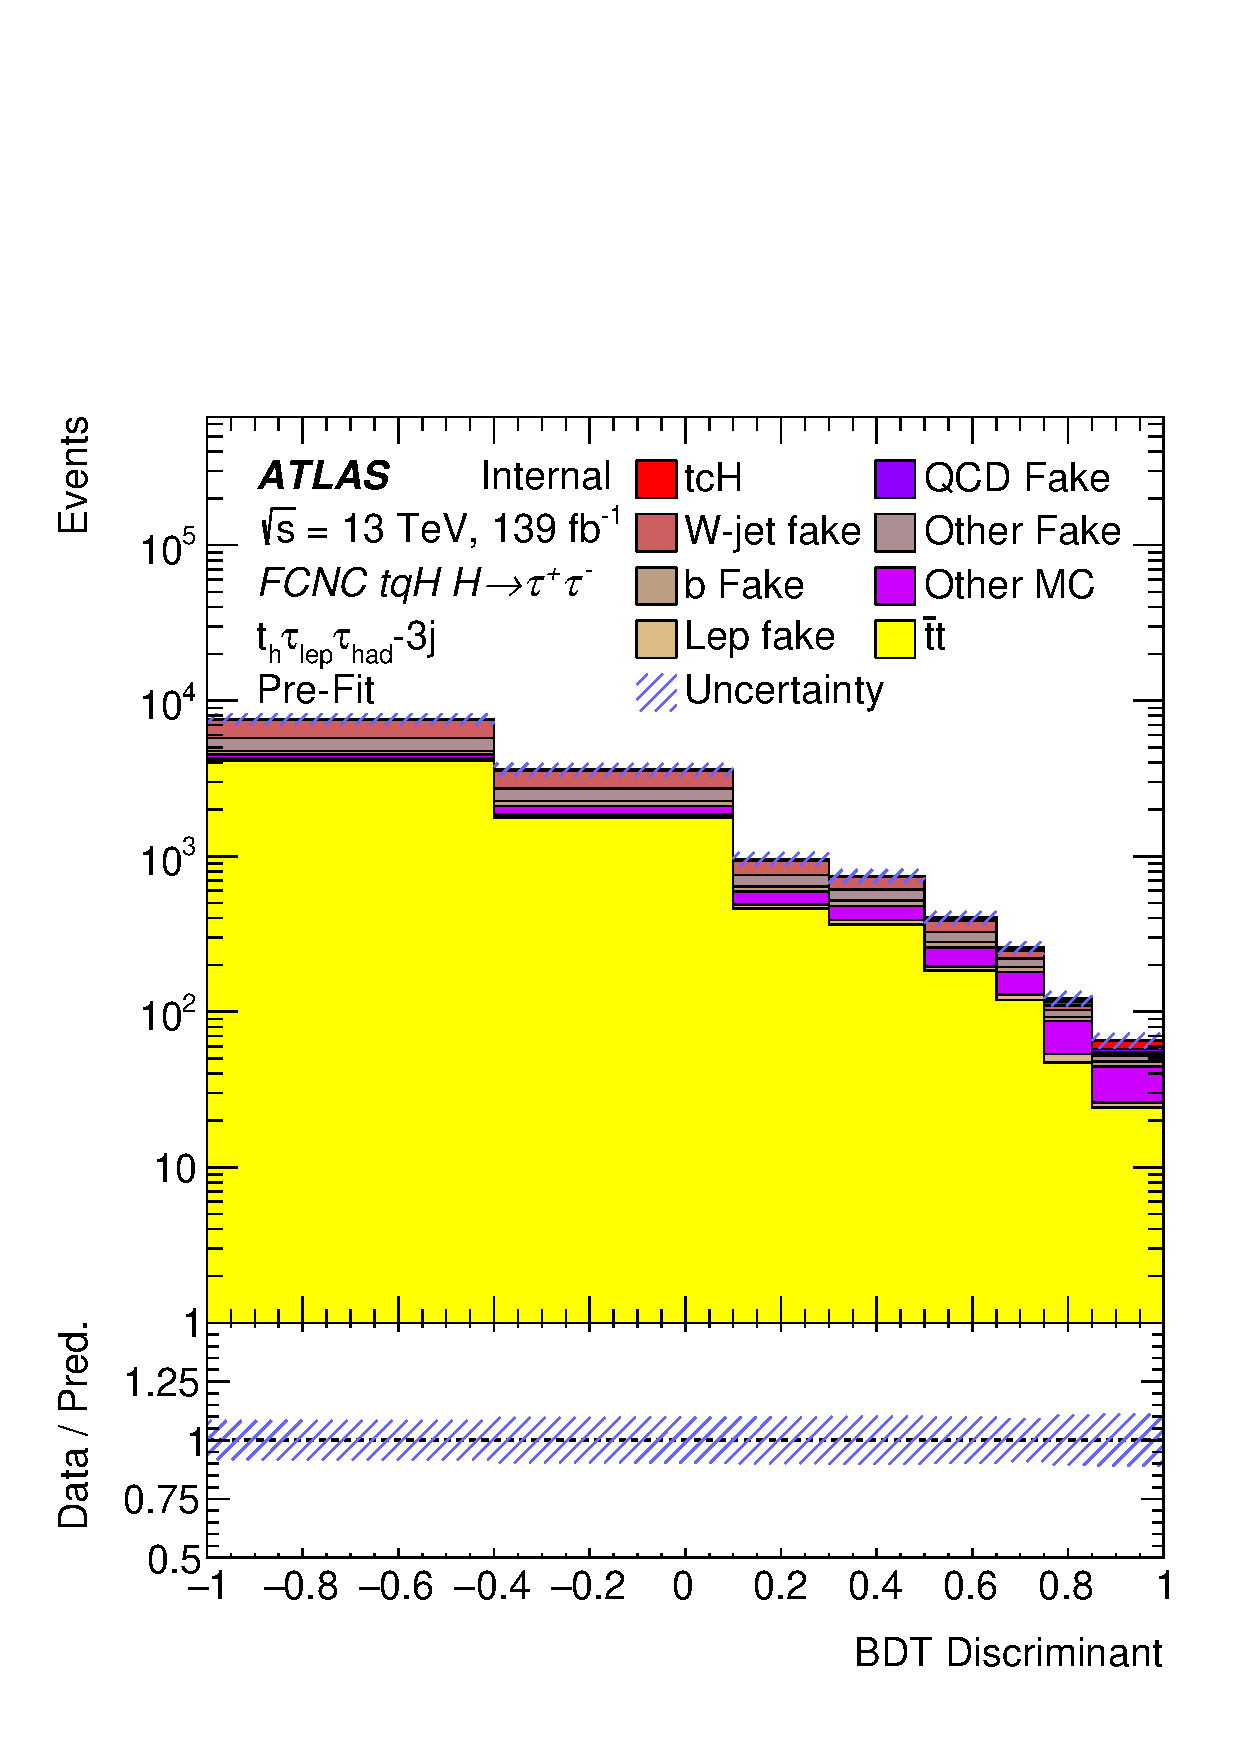
\includegraphics[width=0.30\textwidth]{\FCNCFigures/tthML/Limit/tcH_reg1l1tau1b3j_os.pdf}
\put(-100, 55){\textbf{(b1)}}
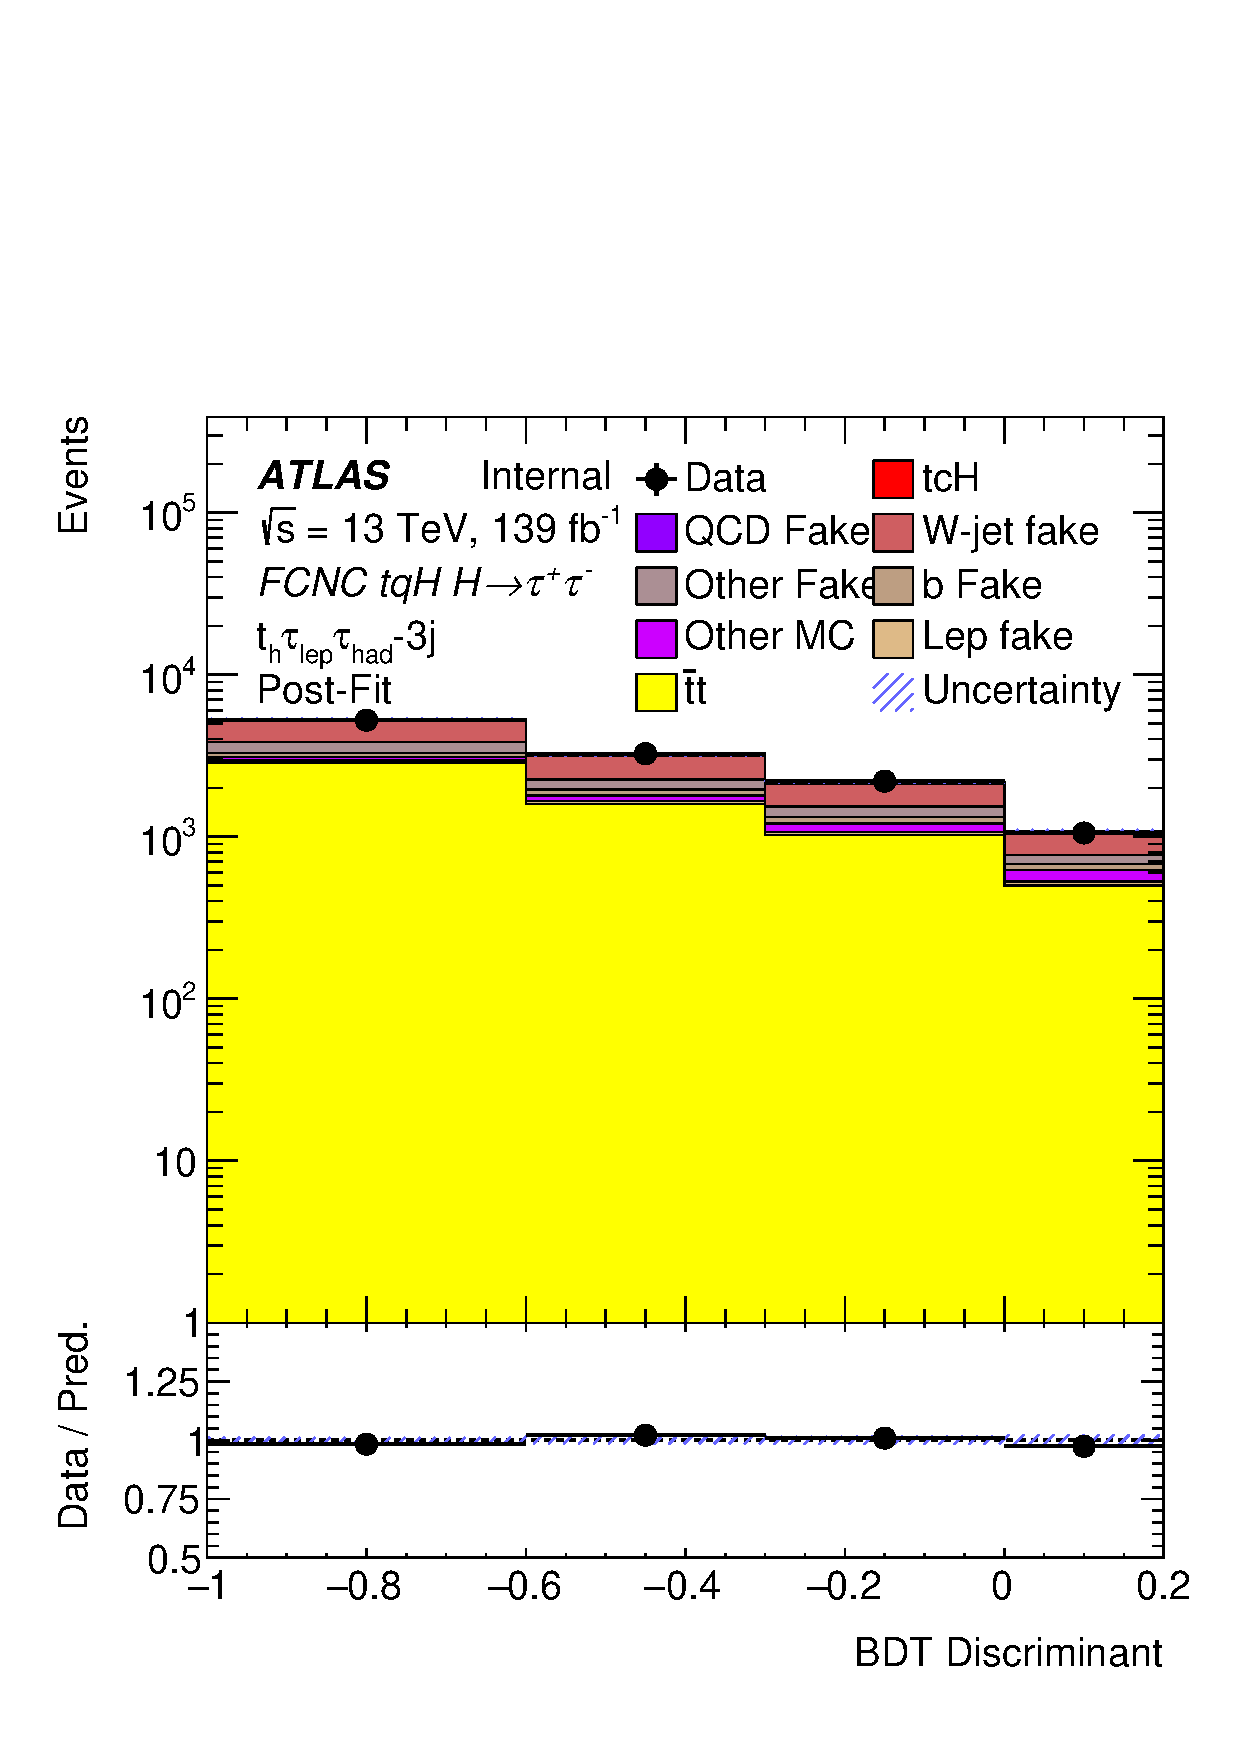
\includegraphics[width=0.30\textwidth]{\FCNCFigures/tthML/Limit/tcH_reg1l1tau1b3j_os_postFit.pdf}
\put(-100, 55){\textbf{(b2)}}
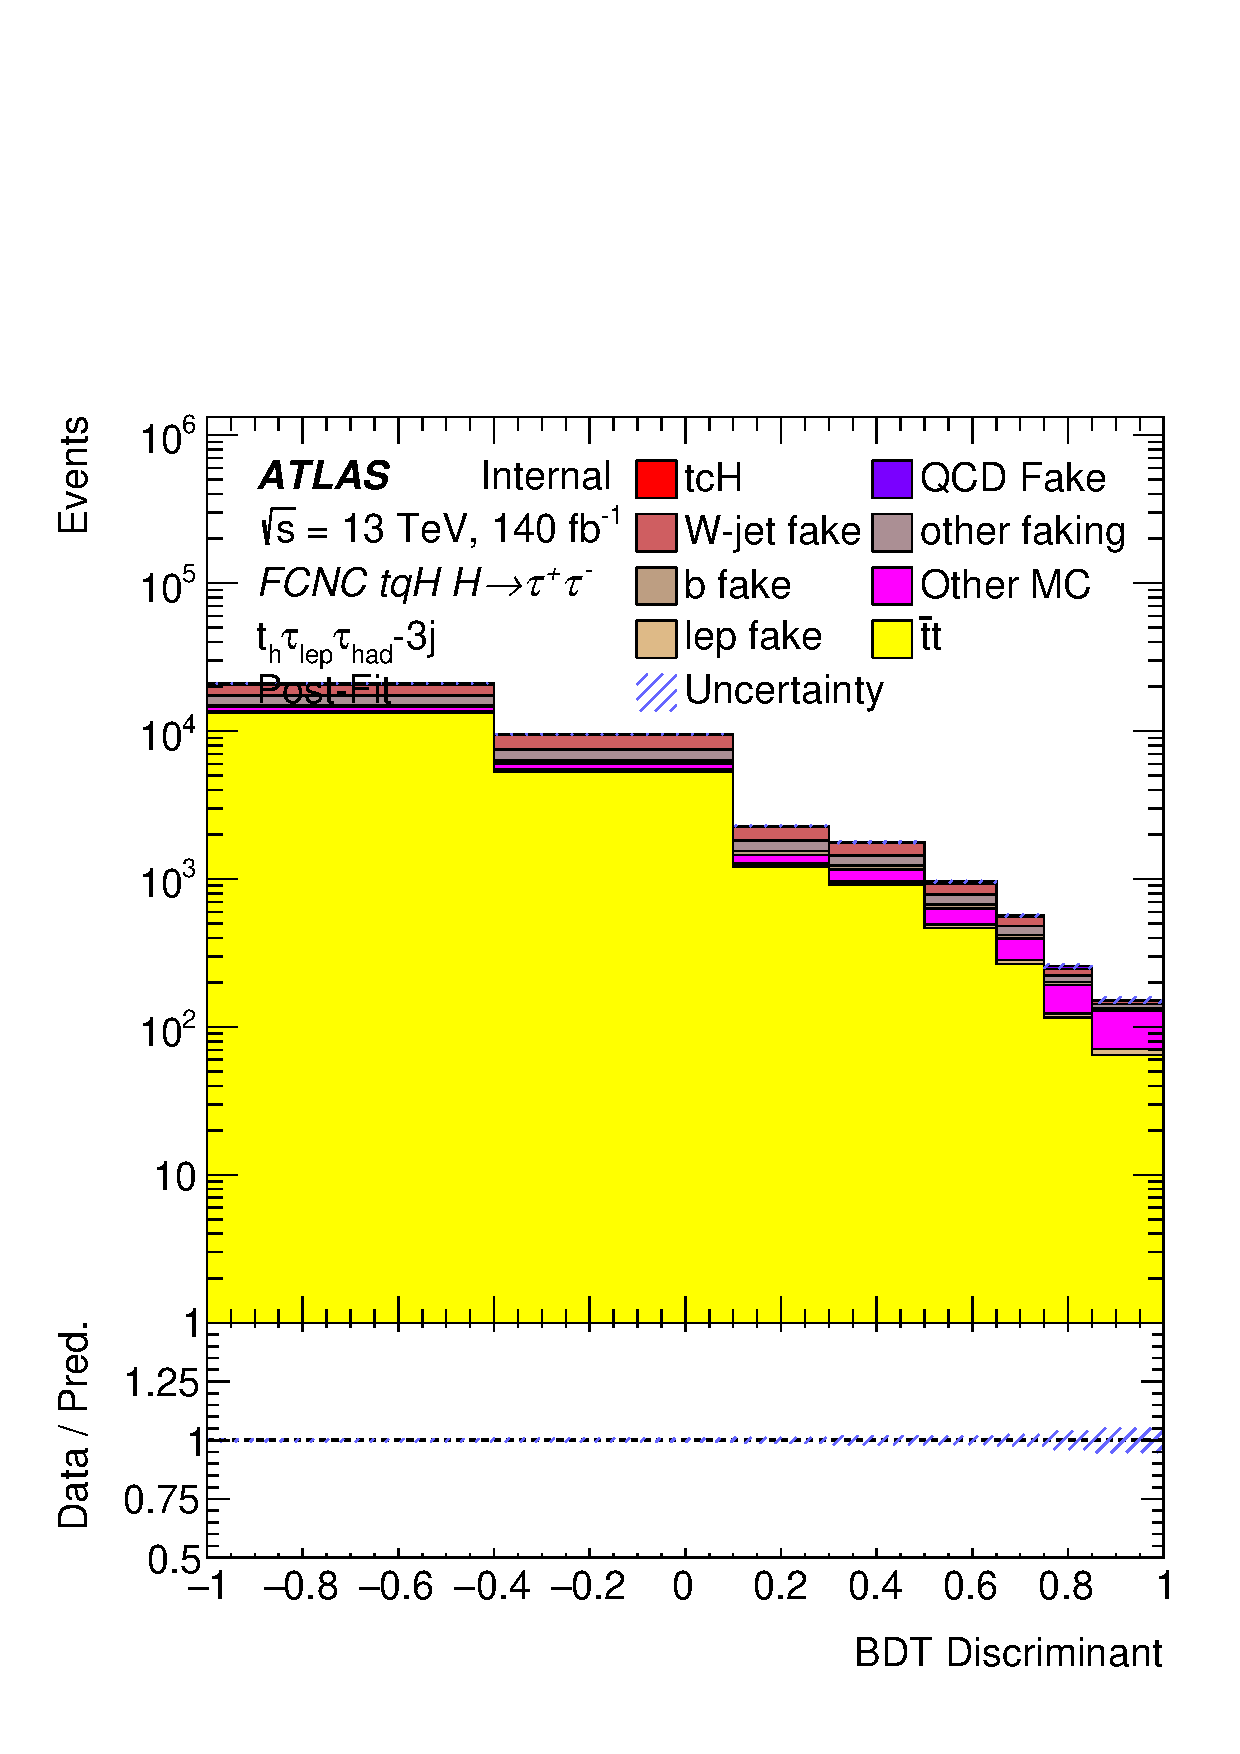
\includegraphics[width=0.30\textwidth]{\FCNCFigures/tthML/Limit/tcH_reg1l1tau1b3j_os_postFit_BOnly.pdf}
\put(-100, 55){\textbf{(b3)}}\\
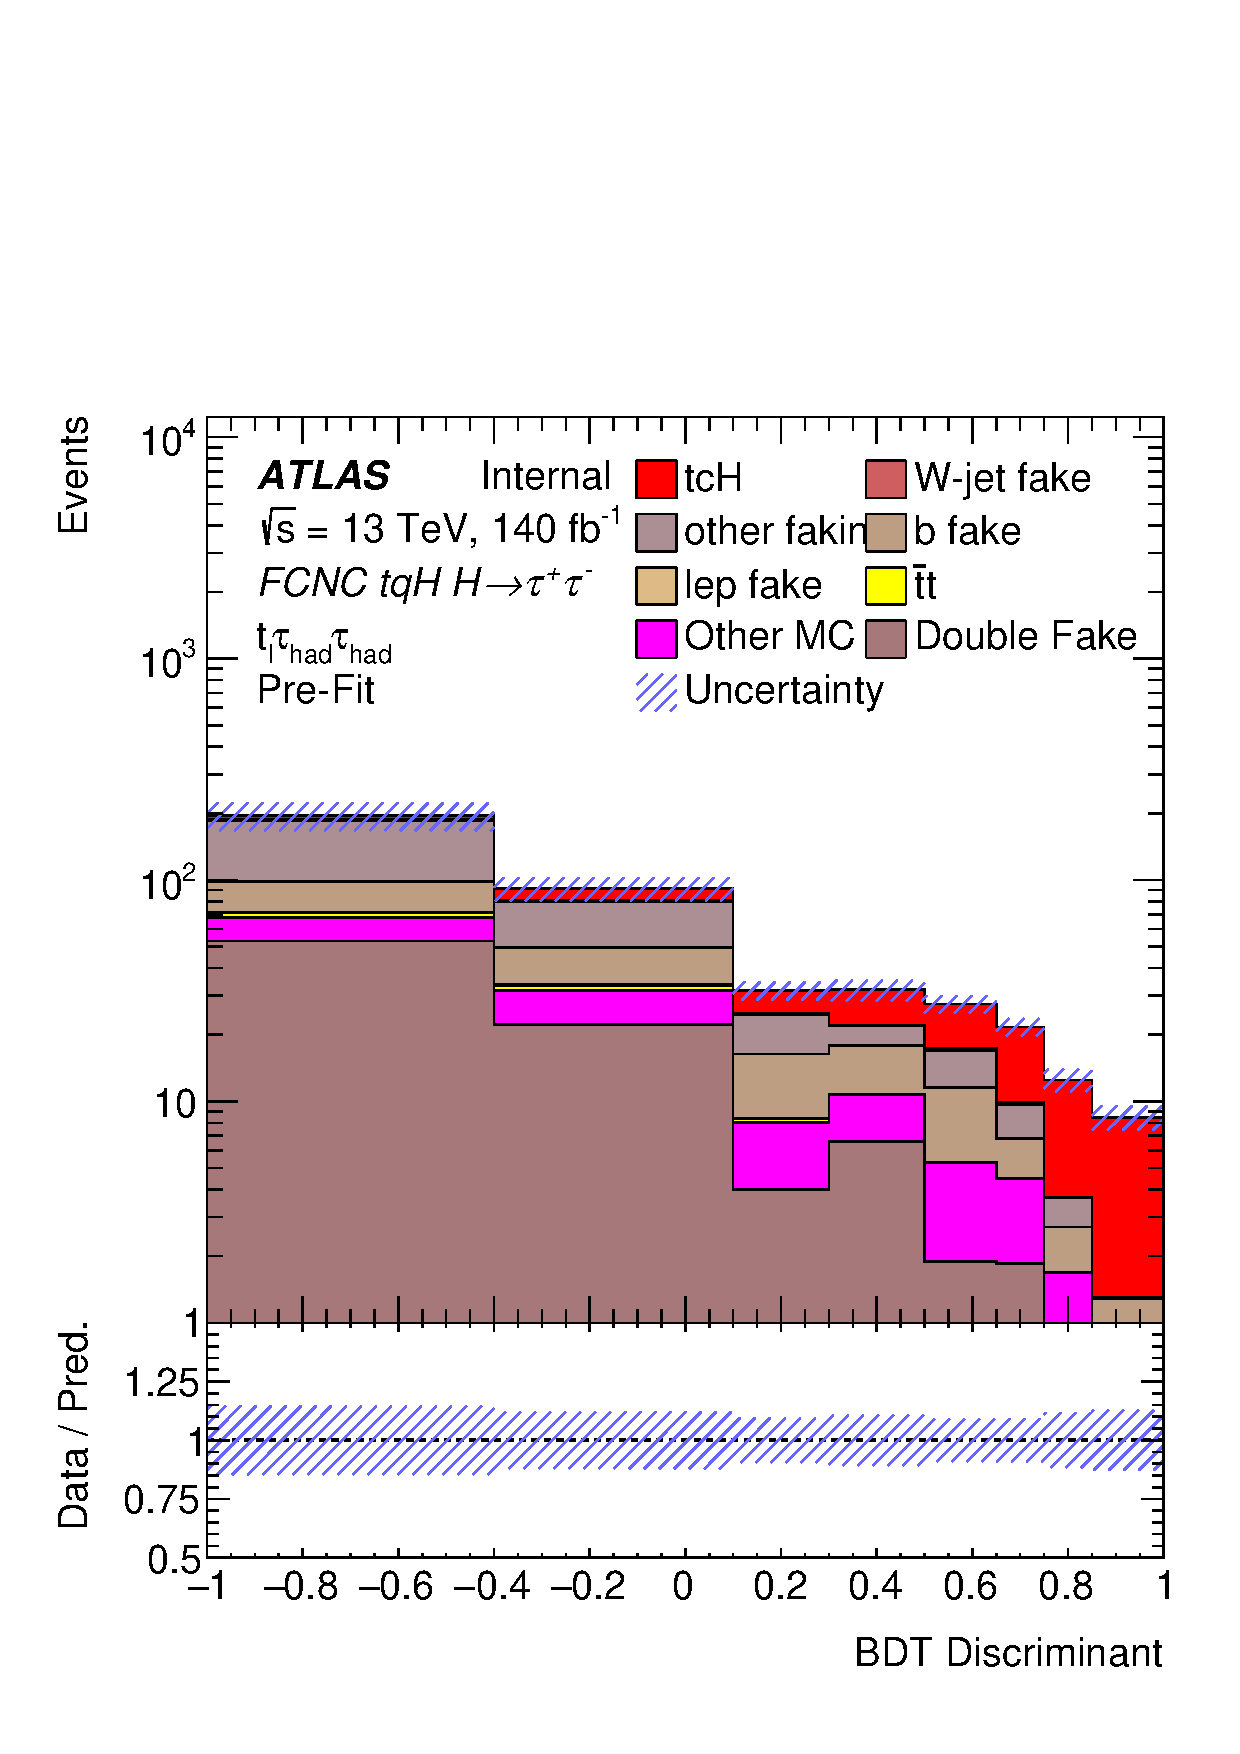
\includegraphics[width=0.30\textwidth]{\FCNCFigures/tthML/Limit/tcH_reg1l2tau1bnj_os.pdf}
\put(-100, 55){\textbf{(c1)}}
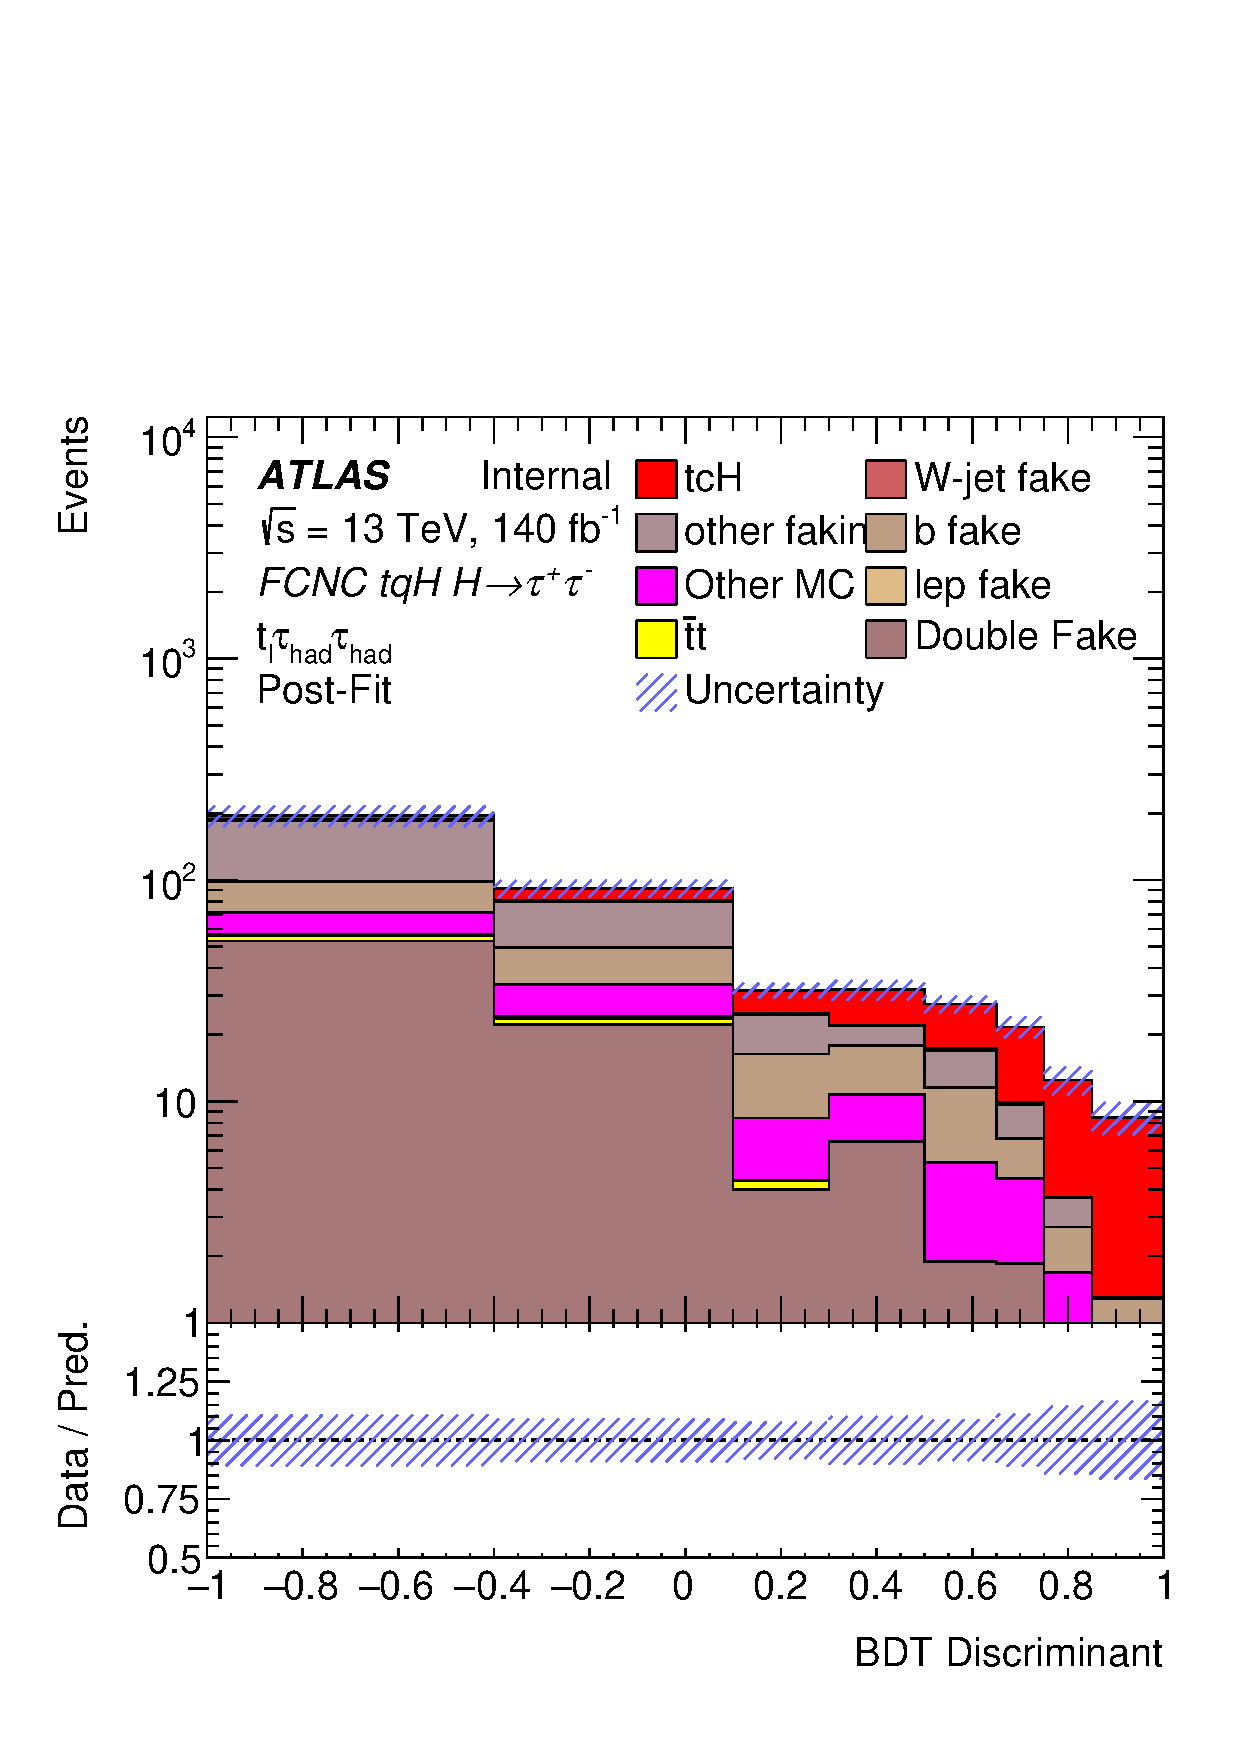
\includegraphics[width=0.30\textwidth]{\FCNCFigures/tthML/Limit/tcH_reg1l2tau1bnj_os_postFit.pdf}
\put(-100, 55){\textbf{(c2)}}
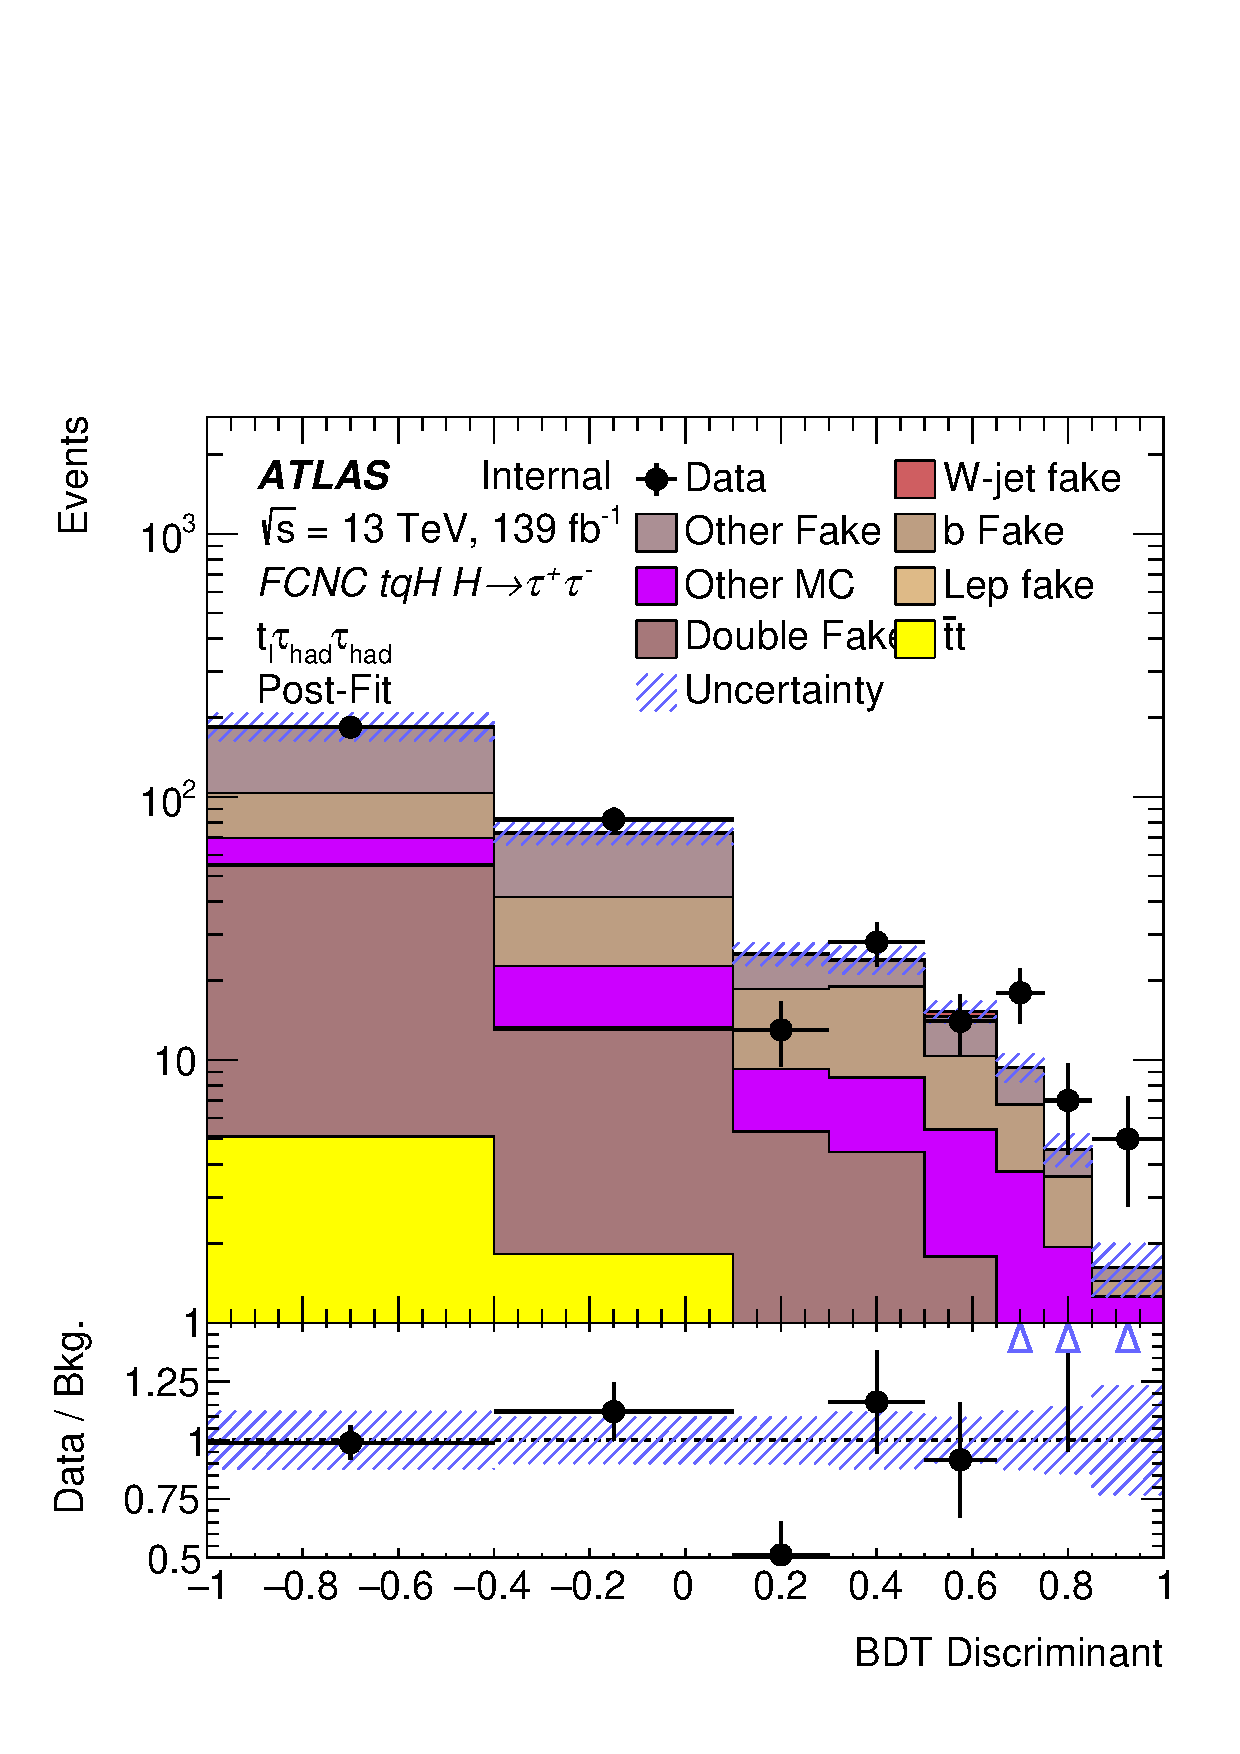
\includegraphics[width=0.30\textwidth]{\FCNCFigures/tthML/Limit/tcH_reg1l2tau1bnj_os_postFit_BOnly.pdf}
\put(-100, 55){\textbf{(c3)}}\\

\caption{ Comparison of the shape of the BDT discriminant distribution between the asimov prefit (a1,b1,c1), asimov postfit  with $\mu$=1 (a2,b2,c2) and background only fit (a3,b3,c3) in terms of tcH merged signal. The upper three plots are in the  $t_h\tlhad$-2j (a1-a3) region, the medium three are in $t_h\tlhad$-3j (b1-b3) and the bottom three are in $t_l\thadhad$ (c1-c3) . Statistical and systematic uncertainties are being shown.}
\label{fig:tthML_trexPrefit_tcH}
\end{figure}

\begin{figure}[H]
\centering
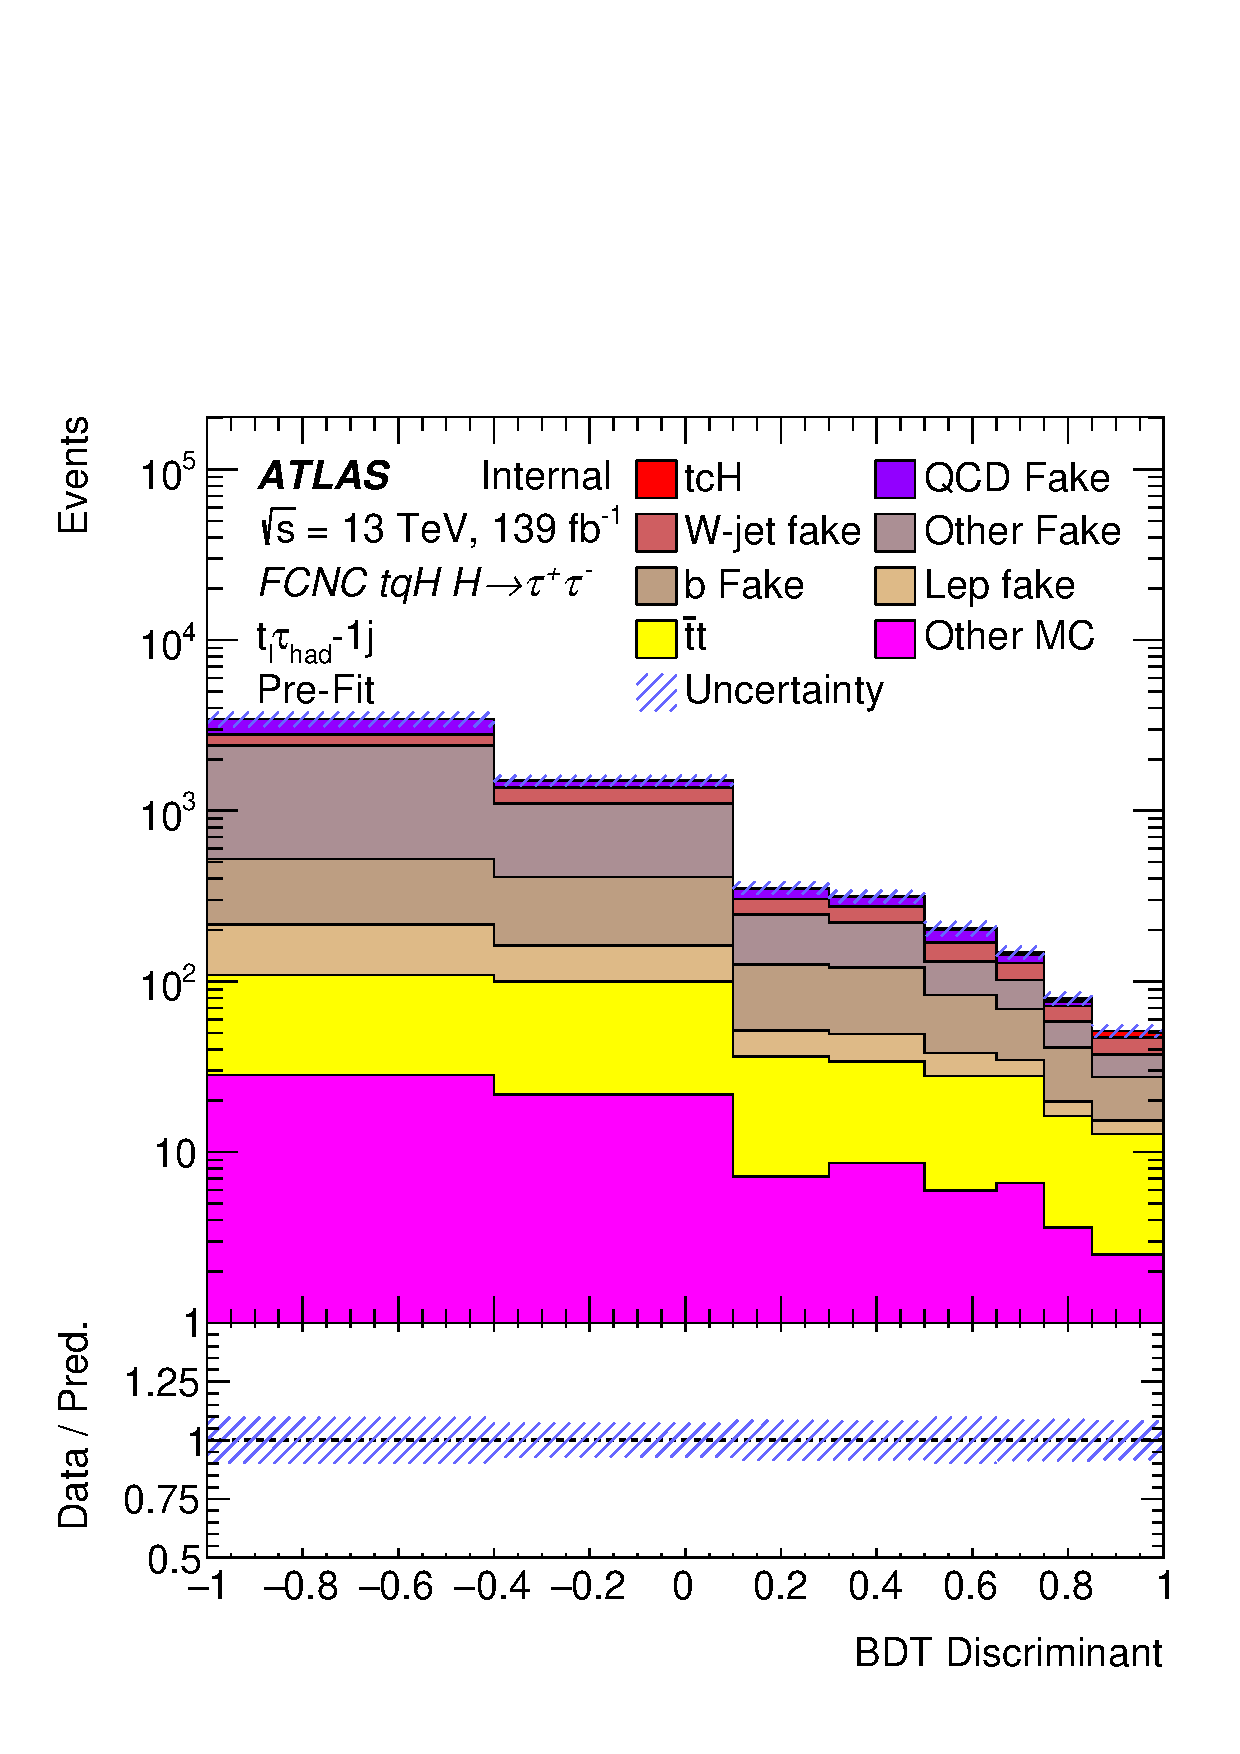
\includegraphics[width=0.30\textwidth]{\FCNCFigures/tthML/Limit/tcH_reg1l1tau1b1j_ss.pdf}
\put(-100, 55){\textbf{(a1)}}
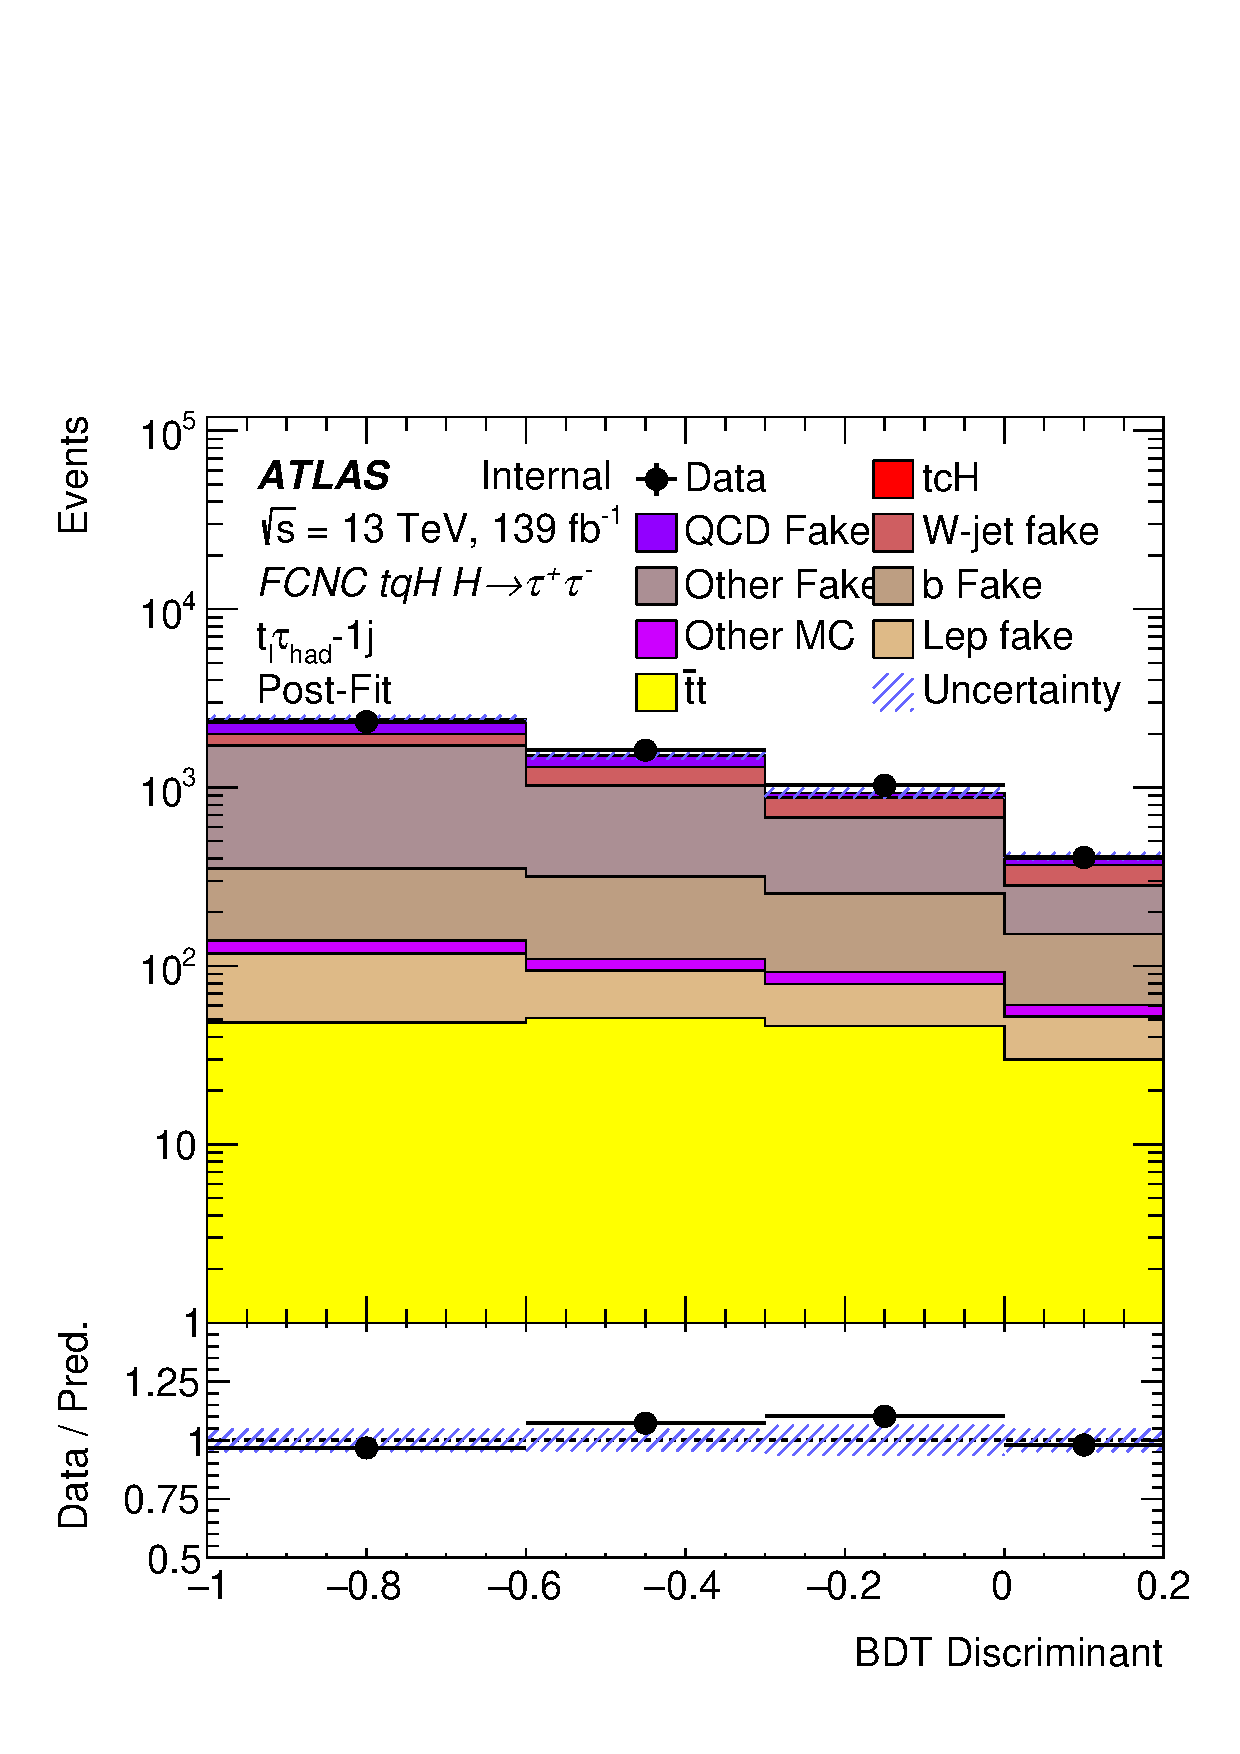
\includegraphics[width=0.30\textwidth]{\FCNCFigures/tthML/Limit/tcH_reg1l1tau1b1j_ss_postFit.pdf}
\put(-100, 55){\textbf{(a2)}}
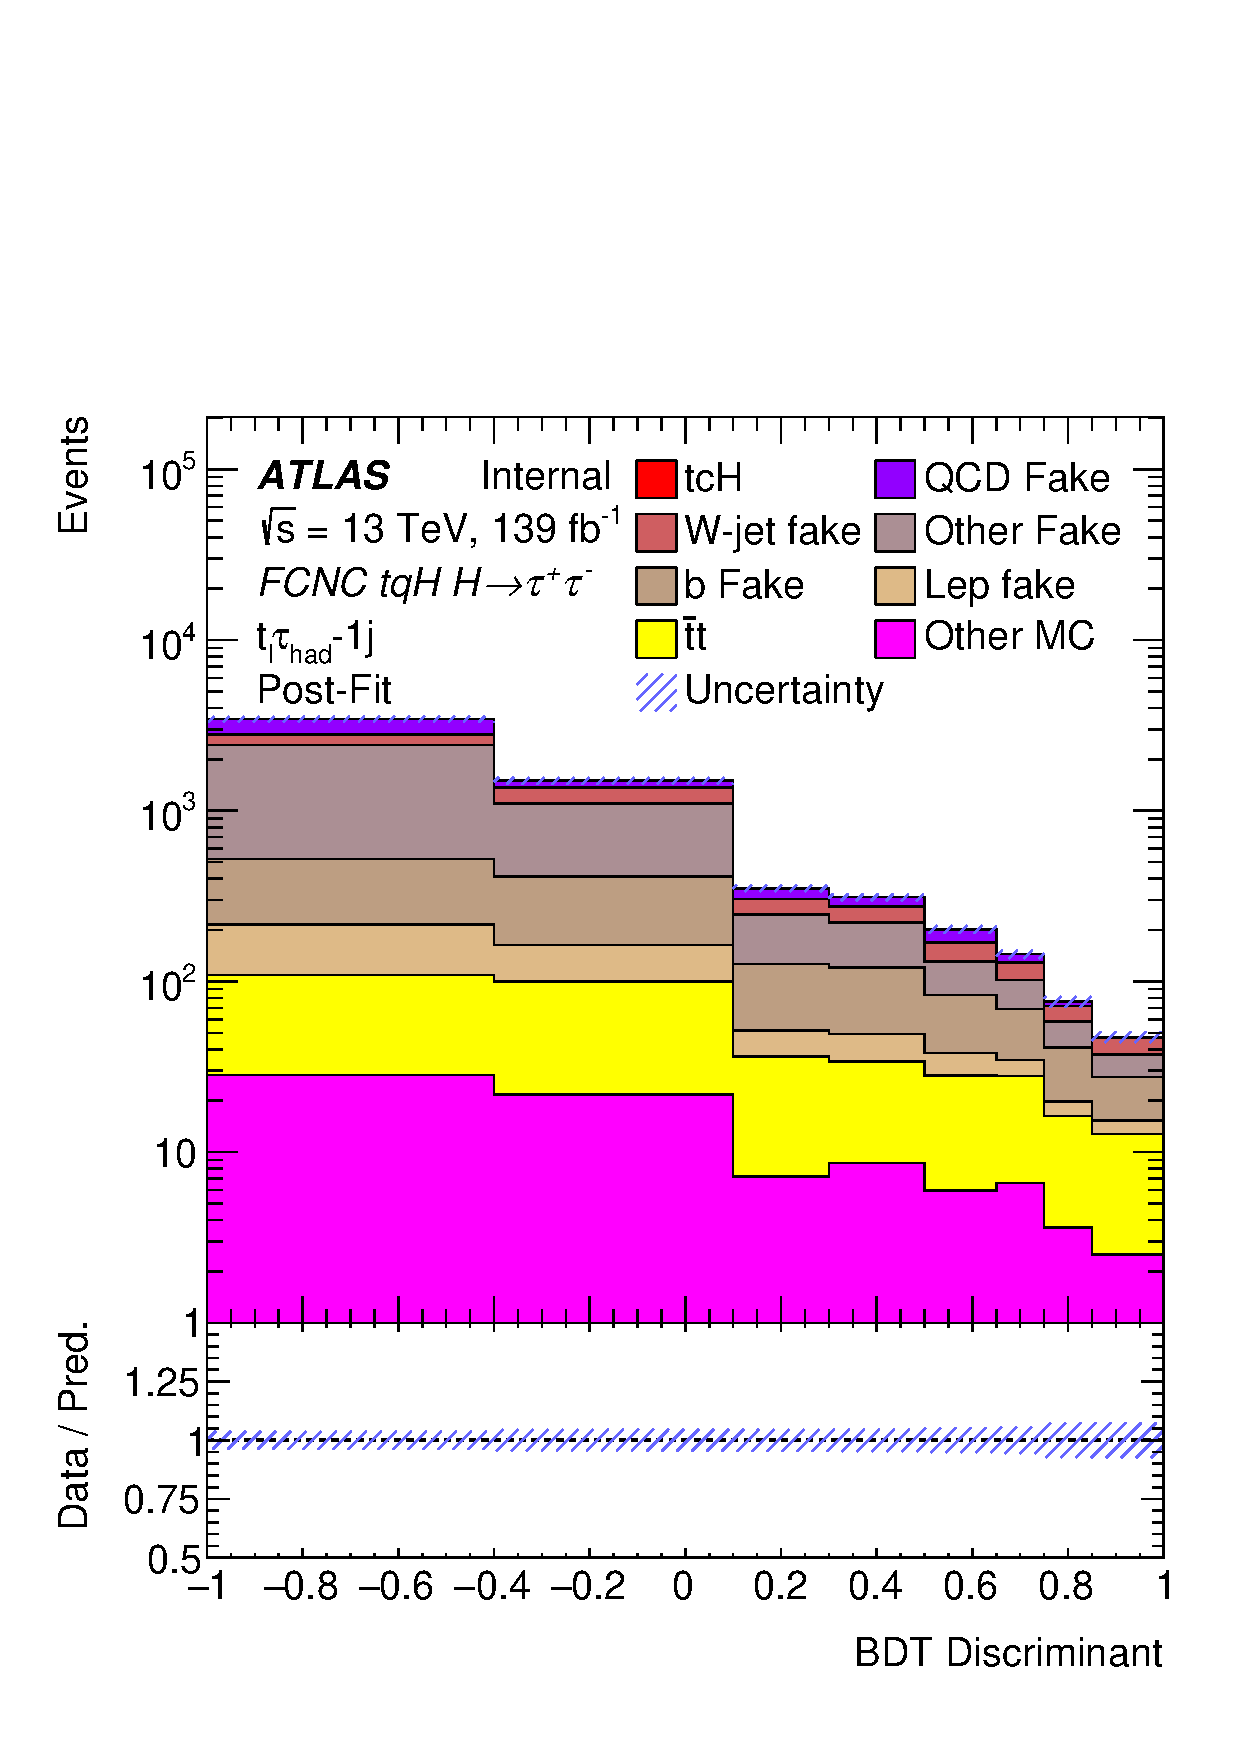
\includegraphics[width=0.30\textwidth]{\FCNCFigures/tthML/Limit/tcH_reg1l1tau1b1j_ss_postFit_BOnly.pdf}
\put(-100, 55){\textbf{(a3)}}\\
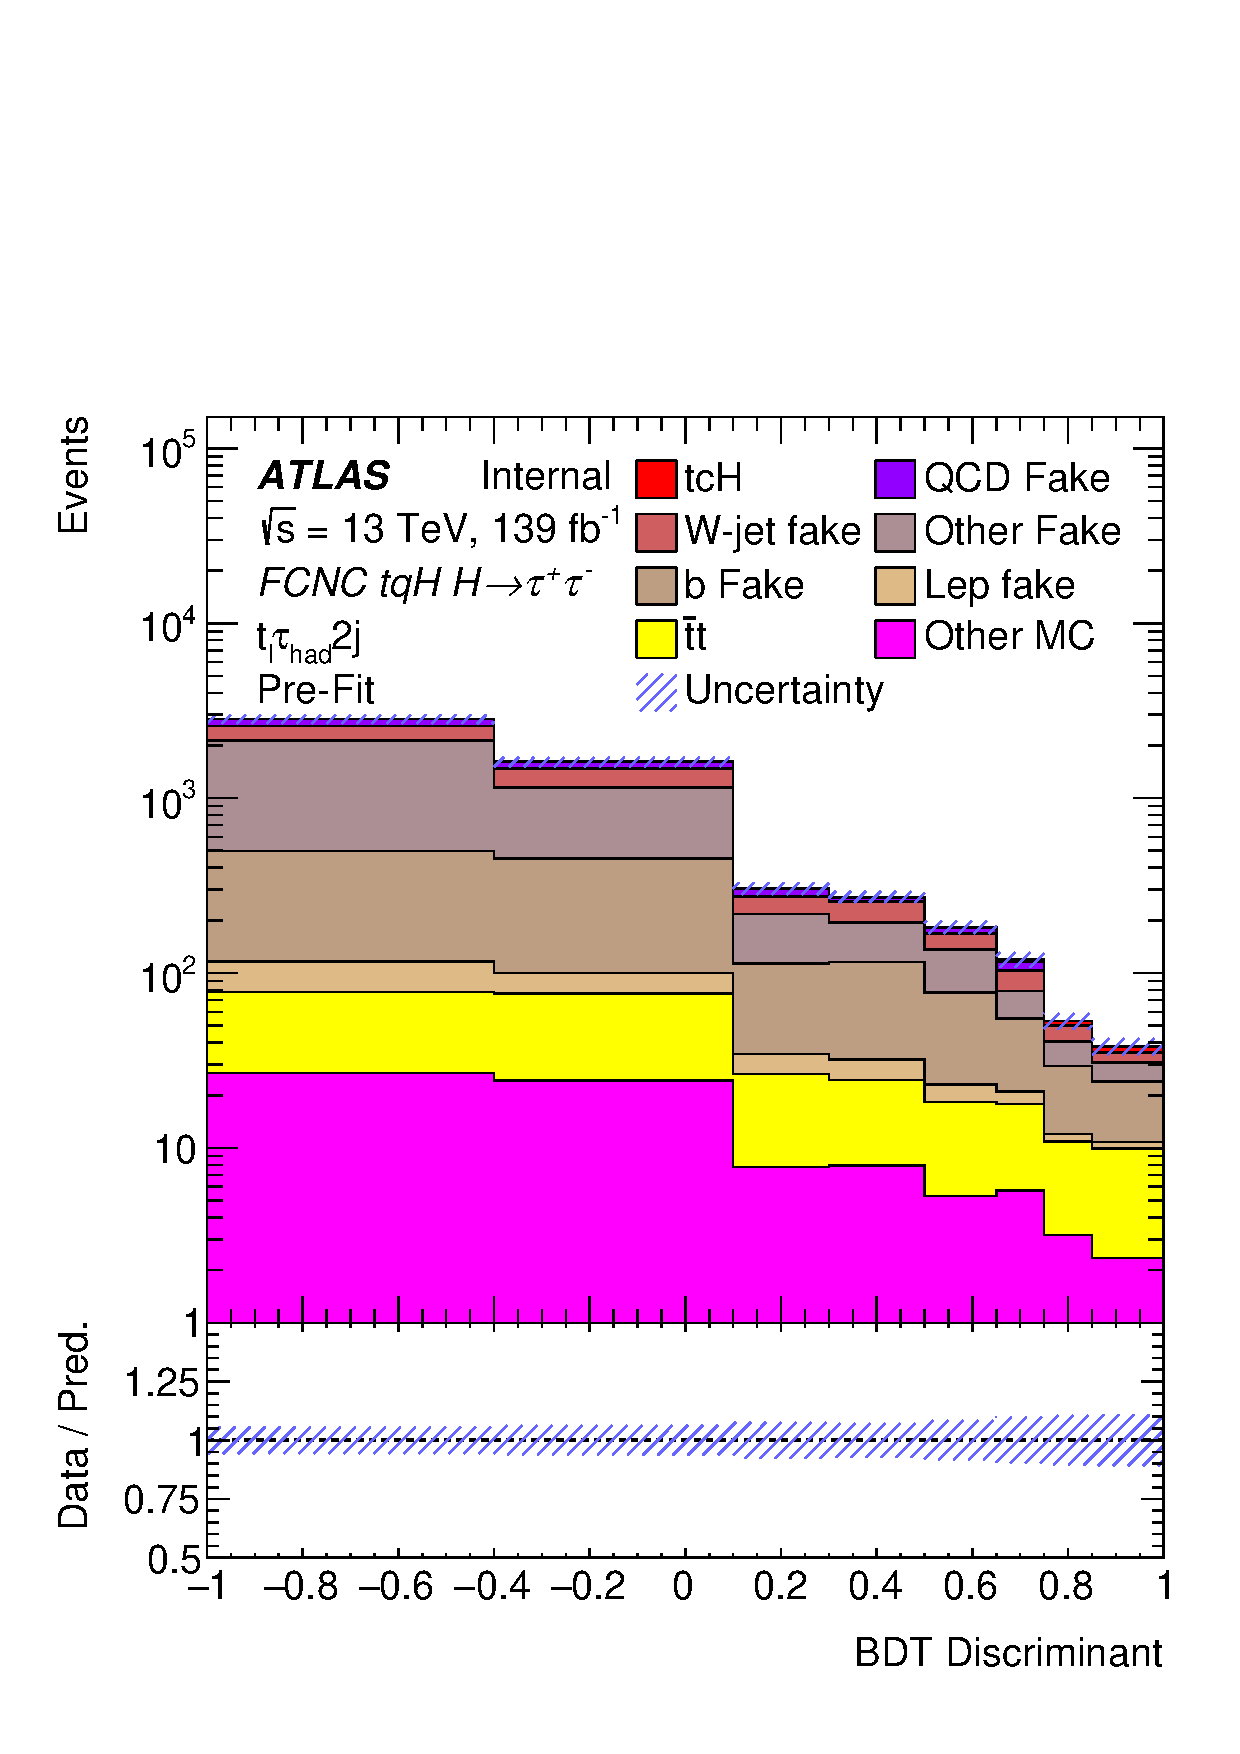
\includegraphics[width=0.30\textwidth]{\FCNCFigures/tthML/Limit/tcH_reg1l1tau1b2j_ss.pdf}
\put(-100, 55){\textbf{(b1)}}
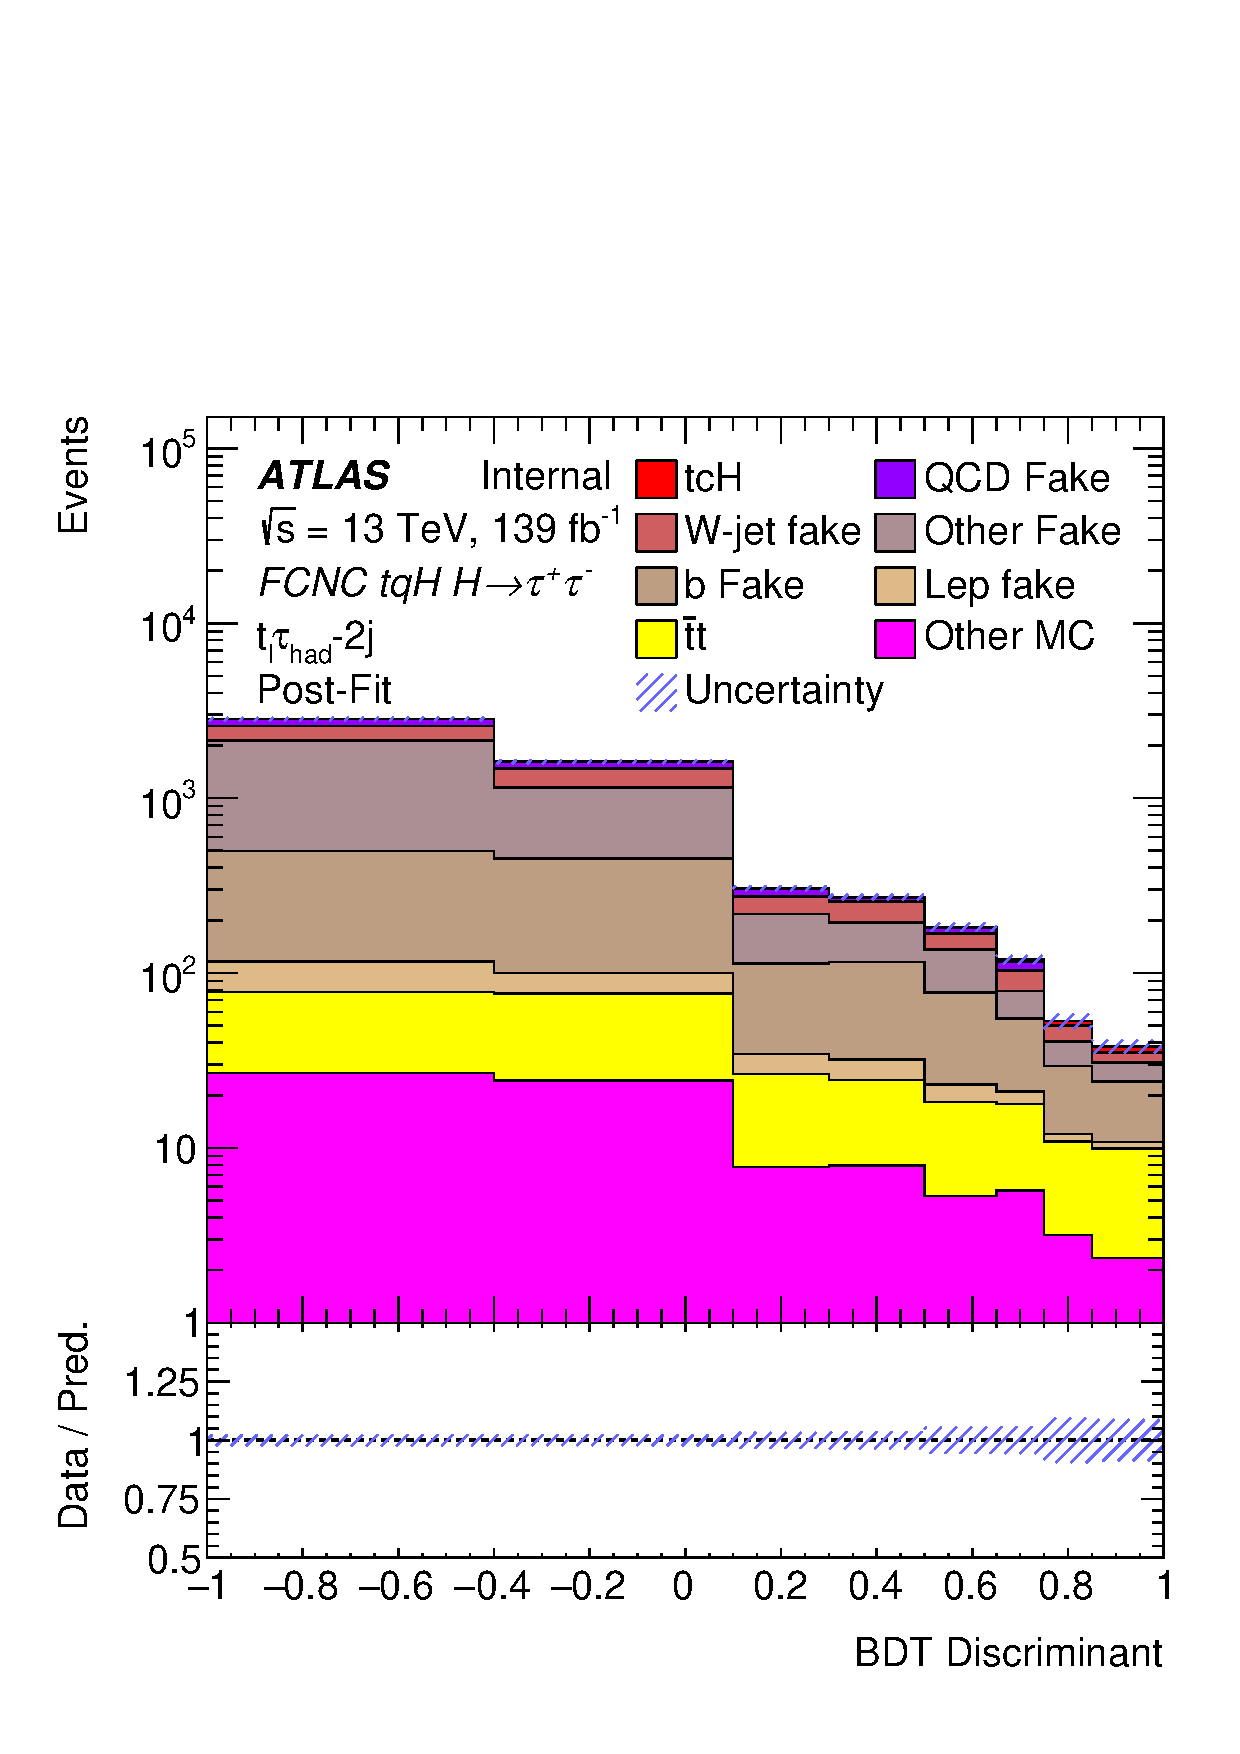
\includegraphics[width=0.30\textwidth]{\FCNCFigures/tthML/Limit/tcH_reg1l1tau1b2j_ss_postFit.pdf}
\put(-100, 55){\textbf{(b2)}}
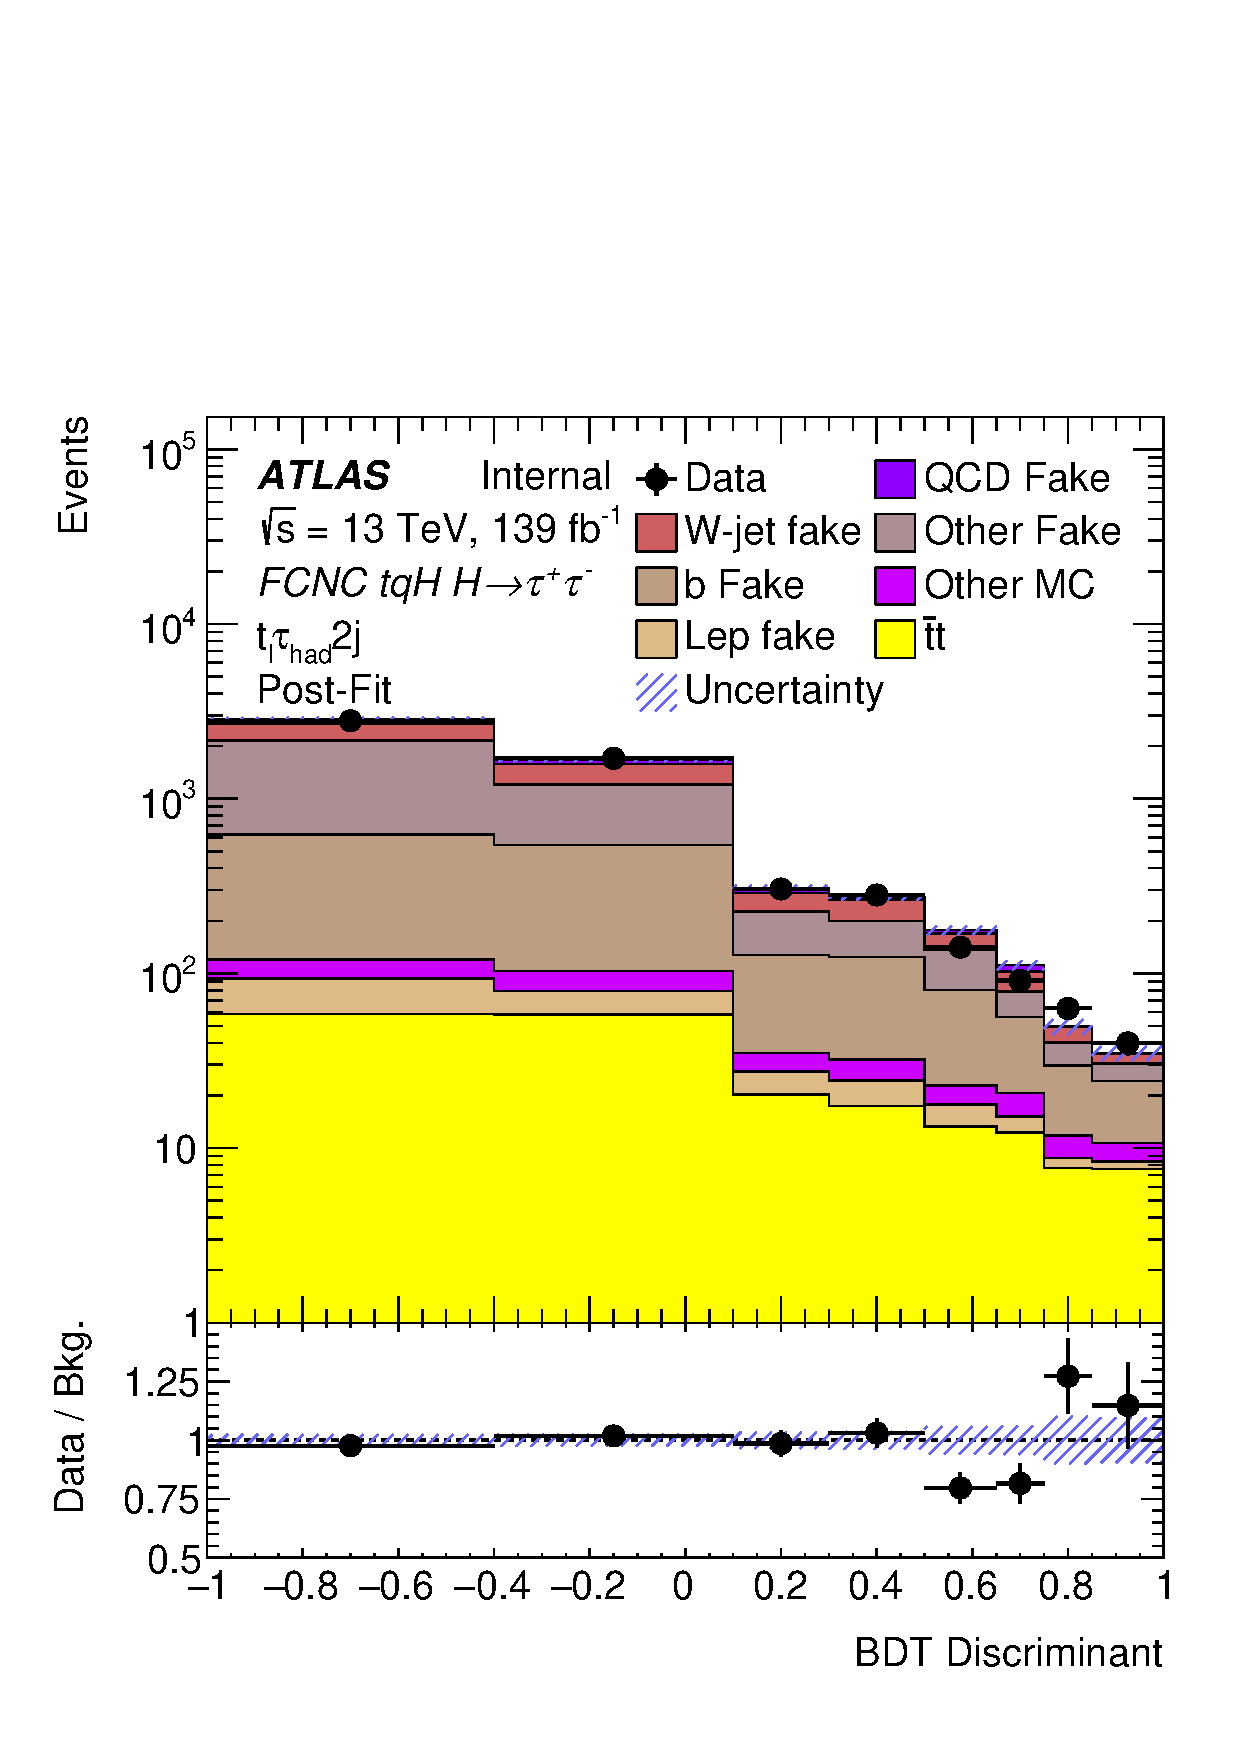
\includegraphics[width=0.30\textwidth]{\FCNCFigures/tthML/Limit/tcH_reg1l1tau1b2j_ss_postFit_BOnly.pdf}
\put(-100, 55){\textbf{(b3)}}\\

\caption{ Comparison of the shape of the BDT discriminant distribution between the asimov prefit (a1,b1), asimov postfit  with $\mu$=1 (a2,b2) and background only fit(a3,b3) in terms of tcH merged signal.The upper three plots are in the  $t_l\tauhad$-1j (a1-a3) region, and the bottom three are in $t_l\tauhad$-2j (b1-b3).Statistical and systematic uncertainties are being shown.}
\label{fig:tthML_trexPrefit_1_tcH}
\end{figure}
